% !TEX program = xelatex
% Науково-популярна версія (15 хв). Детальна наукова версія: main_detailed.tex
\documentclass[aspectratio=169,10pt,t,notheorems]{beamer}
\usetheme{Night}

\usepackage{fontspec}
\usepackage{amsmath,amssymb,mathtools}
\usepackage{unicode-math}
\setsansfont{FiraSans}[Extension=.otf,UprightFont=*-Light,BoldFont=*-SemiBold,
  ItalicFont=*-LightItalic,BoldItalicFont=*-SemiBoldItalic]
\setmainfont{FiraSans}[Extension=.otf,UprightFont=*-Light,BoldFont=*-SemiBold,
  ItalicFont=*-LightItalic,BoldItalicFont=*-SemiBoldItalic]
\setmathfont{Fira Math}
\setmathrm{FiraSans}[Extension=.otf,UprightFont=*-Book,BoldFont=*-SemiBold]
\usepackage[ukrainian]{babel}

\graphicspath{{../figures/}}
% автоматично згенеровано experiments/run_all.py
\newcommand{\lamOne}{0.9058}
\newcommand{\lamTwo}{-0.0003}
\newcommand{\lamThree}{-14.572}
\newcommand{\lamOneErr}{0.0011}
\newcommand{\lamSum}{-13.6667}
\newcommand{\DKY}{2.0621}
\newcommand{\DTwo}{2.072}
\newcommand{\DTwoErr}{0.001}
\newcommand{\rHom}{13.9266}
\newcommand{\rAlo}{24.0578}
\newcommand{\rAhi}{24.0582}
\newcommand{\transGamma}{2.21}
\newcommand{\transGammaErr}{0.14}
\newcommand{\predSlope}{1.096}
\newcommand{\predLam}{0.913}
\newcommand{\predGain}{2.52}
\newcommand{\doublingTime}{0.765}
\newcommand{\lnsixLam}{1.681}
\newcommand{\lnsixNpos}{13}
\newcommand{\lnsixDKY}{27.0}
\newcommand{\lnsixDoubling}{0.41}
\newcommand{\lnsixKS}{10.14}
\newcommand{\enkfRmse}{0.50}
\newcommand{\enkfRmseX}{1.45}
\newcommand{\enkfFree}{10.4}
\newcommand{\orderRK}{4.17}
\newcommand{\orderEuler}{0.97}
\newcommand{\TnumA}{10.4}
\newcommand{\TnumB}{15.7}
\newcommand{\TnumC}{21.6}
\newcommand{\Tnumf}{11.2}
\newcommand{\TnumSlope}{5.04}
\newcommand{\TnumSlopeTh}{4.42}
\newcommand{\ftleNeg}{29}
\newcommand{\regimeMean}{2.32}
\newcommand{\regimeMax}{18}
\newcommand{\mapMinSlope}{1.11}
\newcommand{\butterflyT}{25.3}
\newcommand{\roundErr}{5.8\cdot 10^{-4}}

% автоматично згенеровано experiments/applications.py
\newcommand{\secPct}{4}
\newcommand{\secDecoded}{ХАОС}
\newcommand{\secErr}{0.087}
\newcommand{\secBadDr}{1}
\newcommand{\secMaxOkDr}{0.1}
\newcommand{\wheelLam}{0.492}
\newcommand{\wheelRev}{132}
\newcommand{\wheelHopf}{17.5}
\newcommand{\esnVT}{9.6}
\newcommand{\esnVTmin}{4.1}
\newcommand{\esnVTmax}{15.6}
\newcommand{\esnTrain}{181}
\newcommand{\sinSigma}{10.000}
\newcommand{\sinRho}{28.000}
\newcommand{\sinBeta}{2.667}
\newcommand{\sinNSigma}{10.01}
\newcommand{\sinNRho}{27.90}
\newcommand{\sinNBeta}{2.66}
\newcommand{\sinWSigma}{10.00}
\newcommand{\sinWRho}{28.00}
\newcommand{\sinWBeta}{1.00}


\newcommand{\Div}{\operatorname{div}}
\newcommand{\norm}[1]{\lVert #1\rVert}

\title{Ефект метелика}
\author{Сучок Катерина, Шопська Анастасія, Бугір Єлизавета}
\date{2026}

\begin{document}

% =====================================================================
% 1. ТИТУЛ
% =====================================================================
{\setbeamertemplate{footline}{}
\setbeamertemplate{background canvas}{}
\begin{frame}[plain]
  \begin{tikzpicture}[remember picture,overlay]
    \fill[NNight] (current page.south west) rectangle (current page.north east);
    \node[opacity=0.55,inner sep=0] at (current page.center)
      {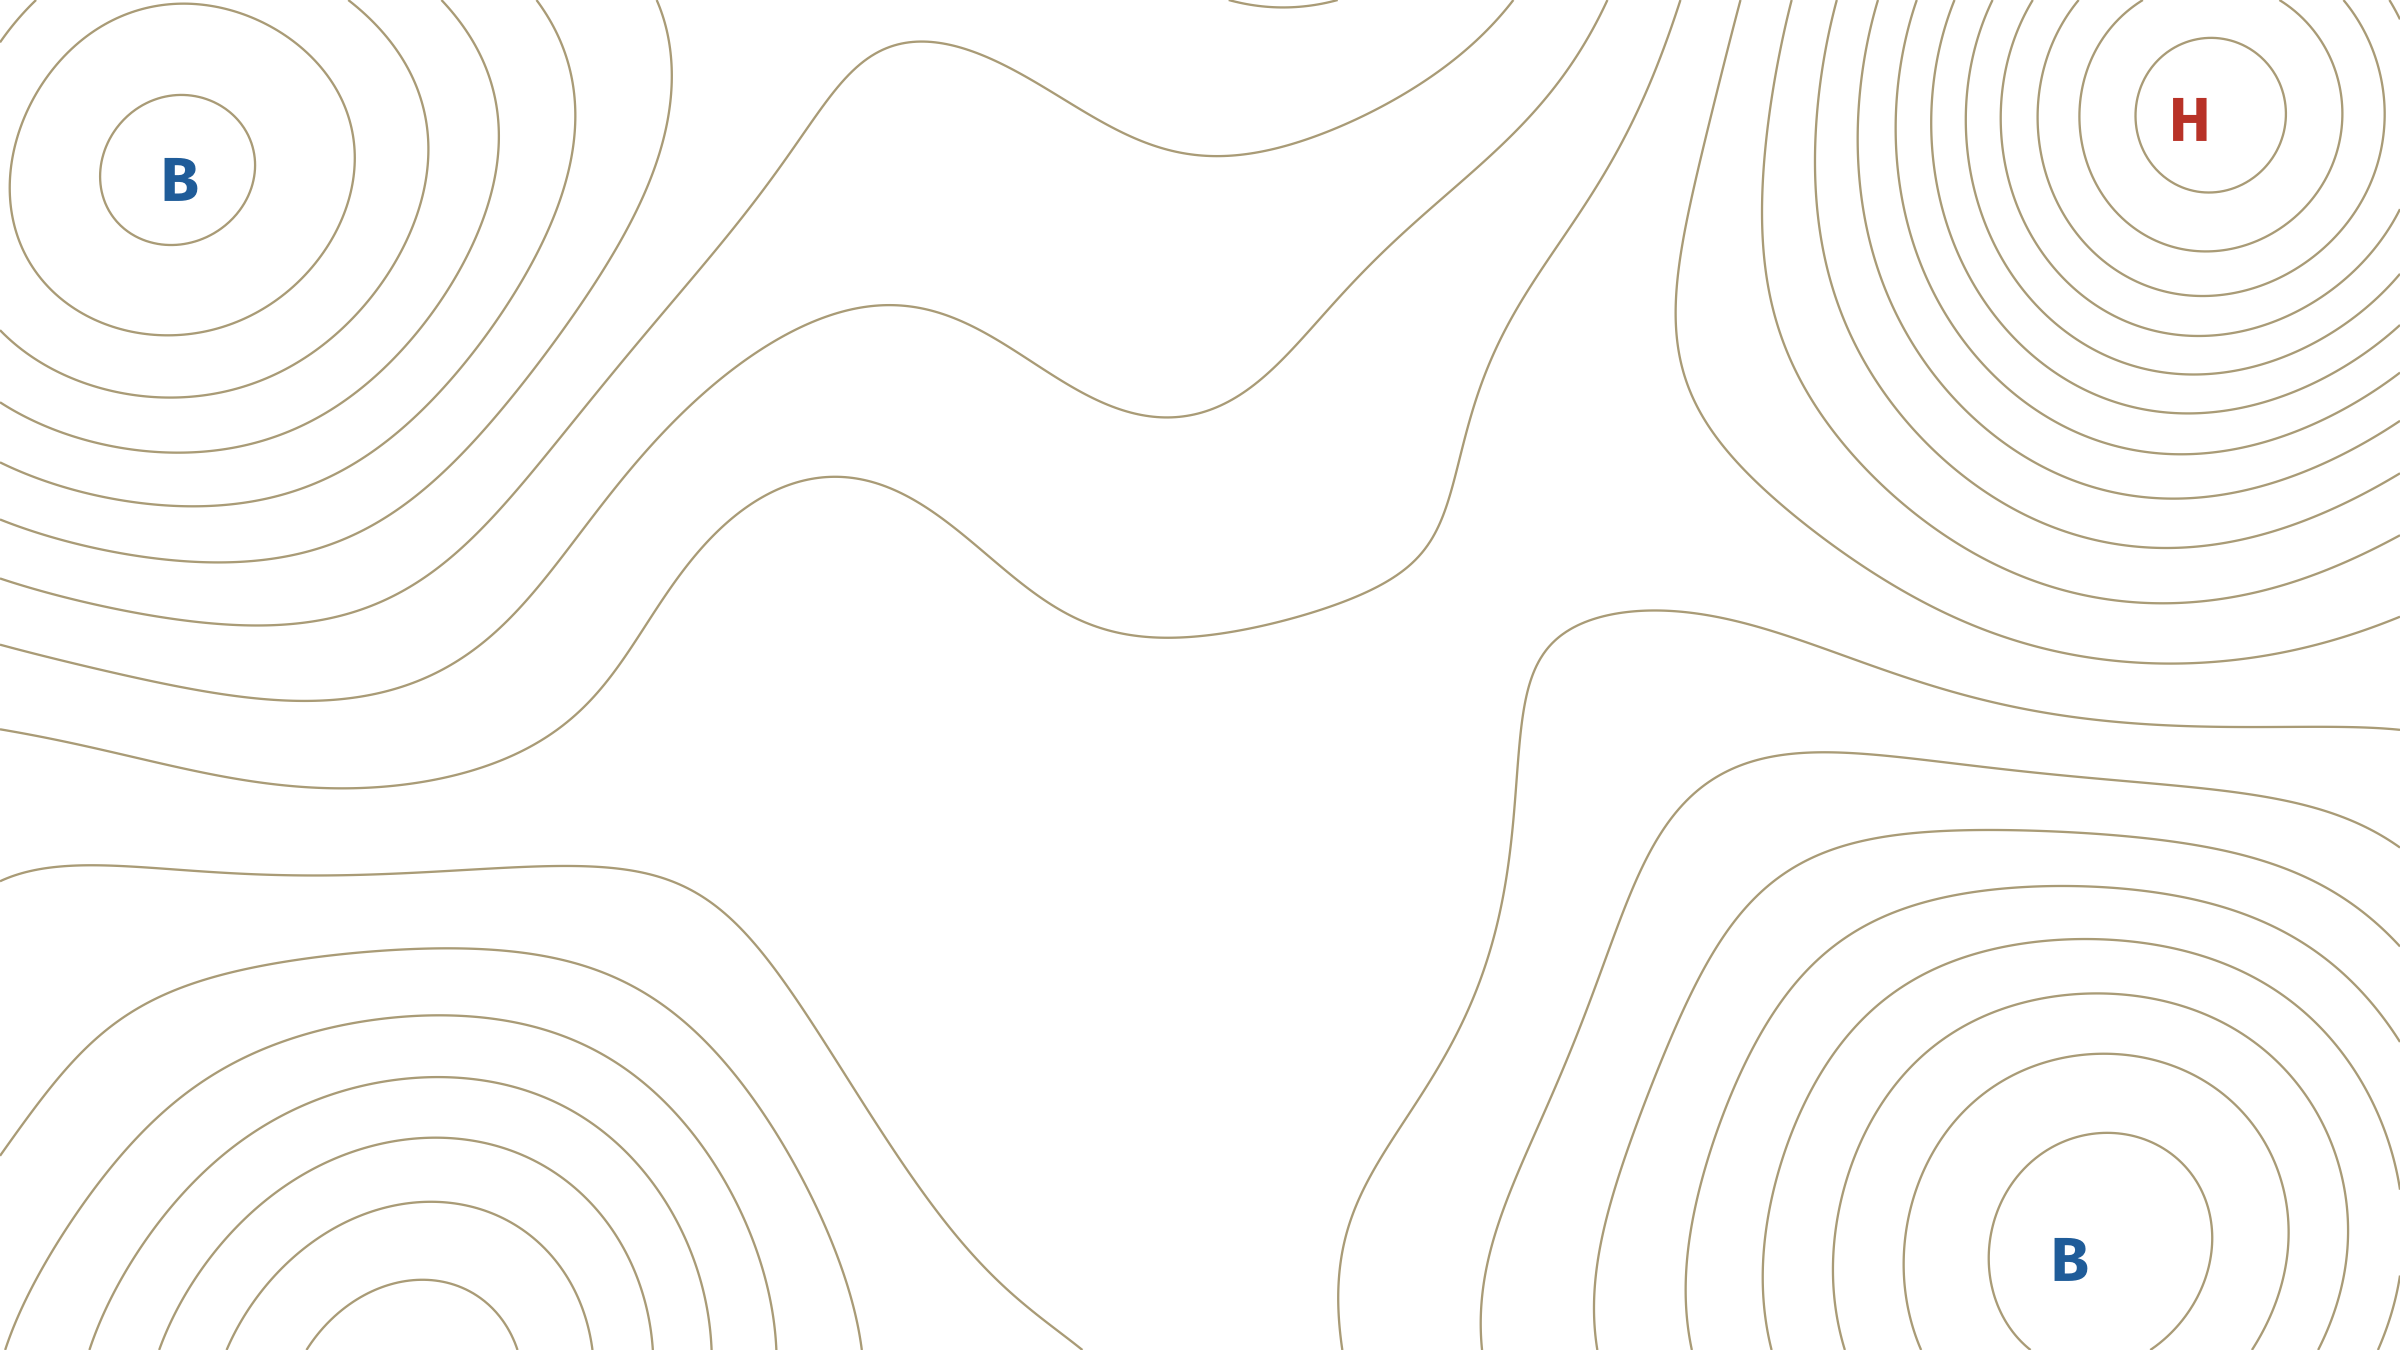
\includegraphics[width=\paperwidth,height=\paperheight]{pop_isobars_title.png}};
    \node[anchor=east,inner sep=0] at ($(current page.east)+(-0.3,-0.2)$)
      {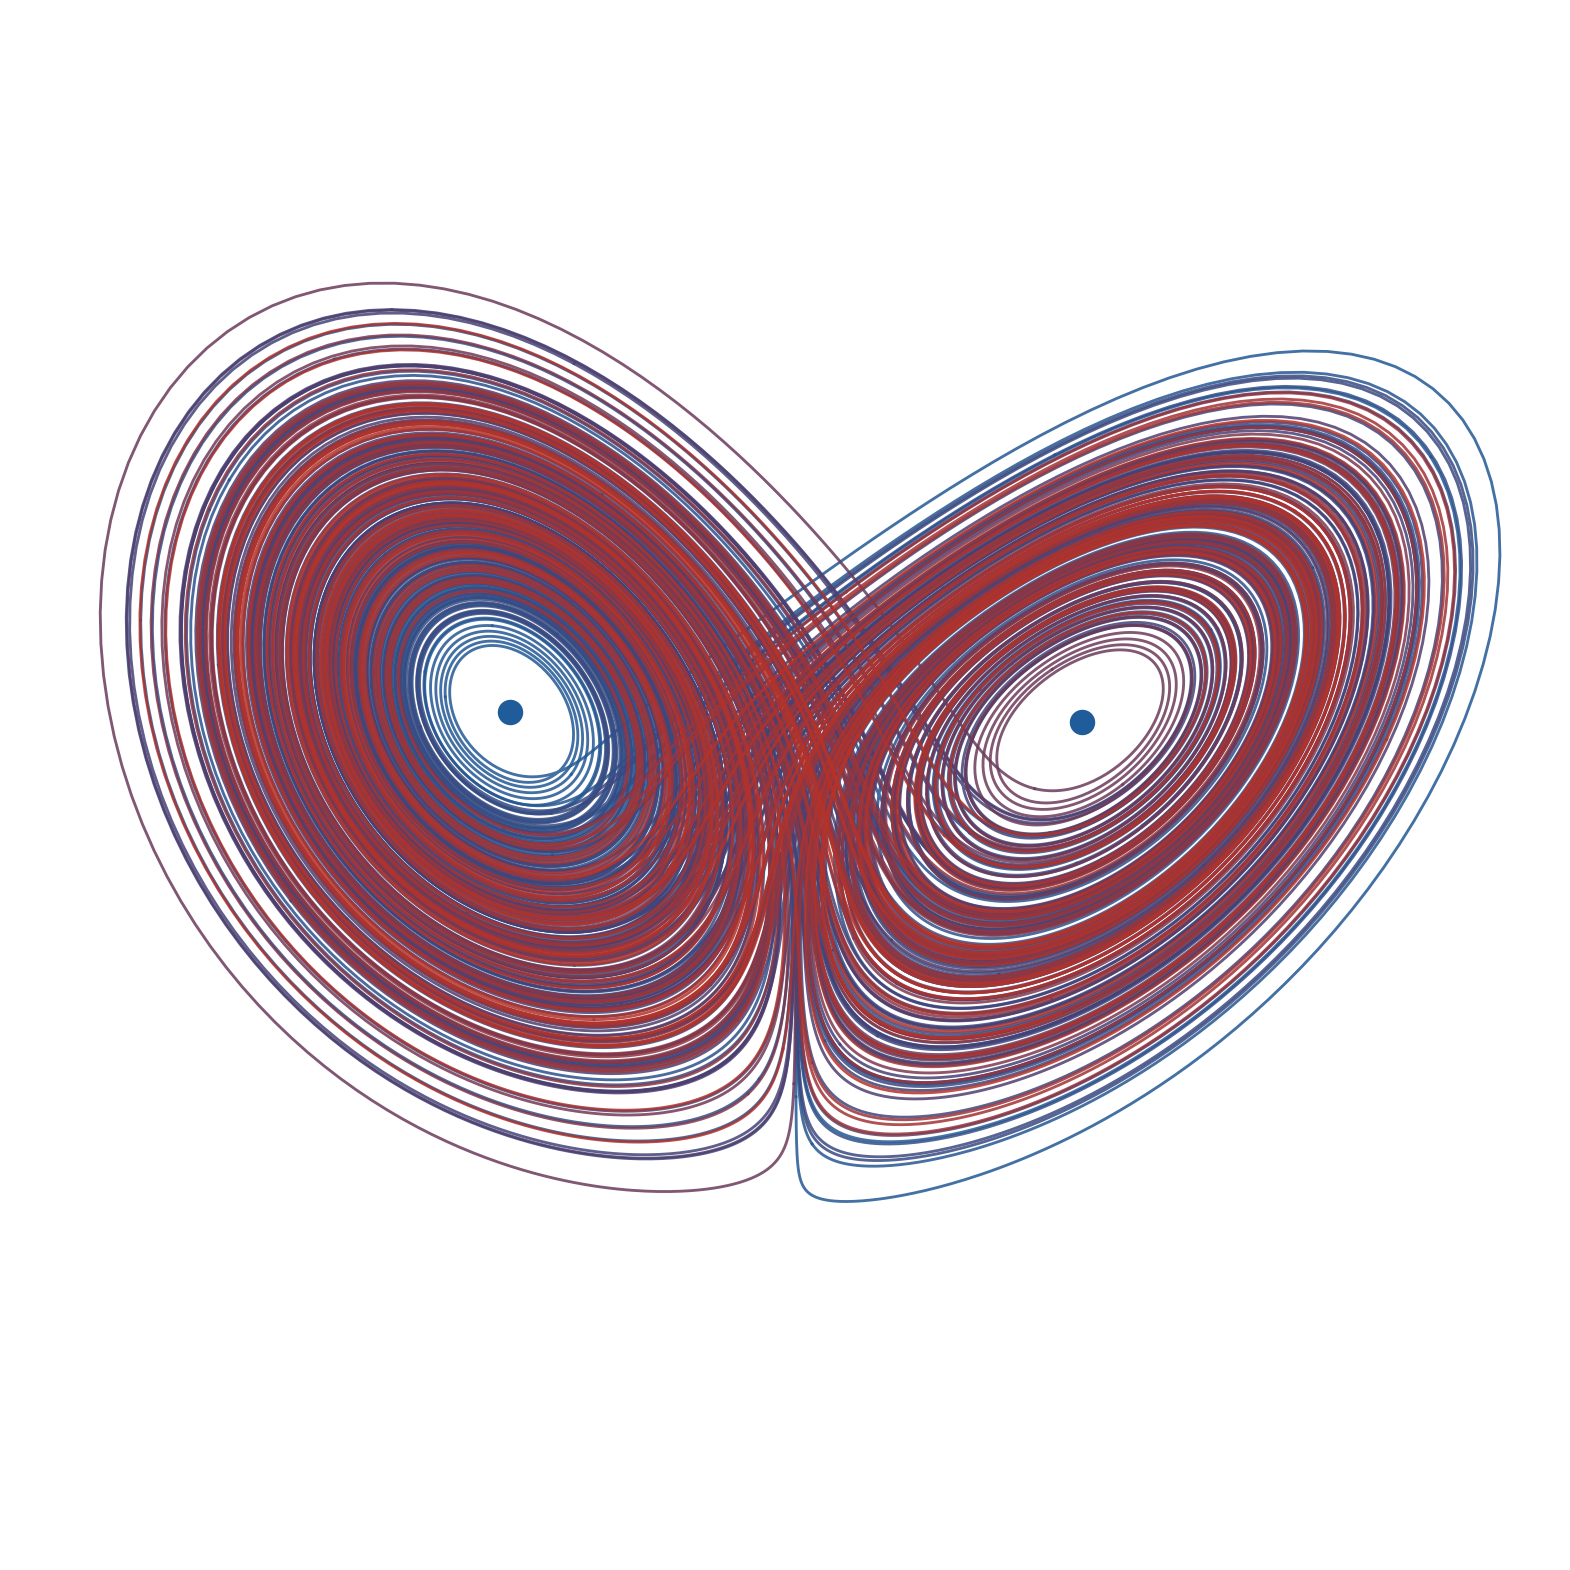
\includegraphics[height=0.82\paperheight]{pop_attractor.png}};
    \node[anchor=north west,font=\fontsize{38}{42}\selectfont\bfseries,text=NInk]
      at ($(current page.north west)+(0.85,-1.7)$) {Ефект метелика};
    \node[anchor=north west,inner sep=0] at ($(current page.north west)+(0.95,-3.1)$) {\Nfront};
    \node[anchor=north west,text=NInk,font=\Large,align=left]
      at ($(current page.north west)+(0.85,-3.55)$) {Дивний атрактор Лоренца\\ та детермінований хаос};
    \node[anchor=south west,text=NInk,font=\normalsize,align=left]
      at ($(current page.south west)+(0.85,0.7)$) {\textbf{Сучок Катерина}\\ \textbf{Шопська Анастасія}\\ \textbf{Бугір Єлизавета}\\ \textcolor{NDim}{Динамічні системи, 2026}};
  \end{tikzpicture}
\end{frame}}

% =====================================================================
% 2. ІСТОРІЯ
% =====================================================================
\begin{frame}{Дослід Лоренца, 1961 рік}
  \centering
  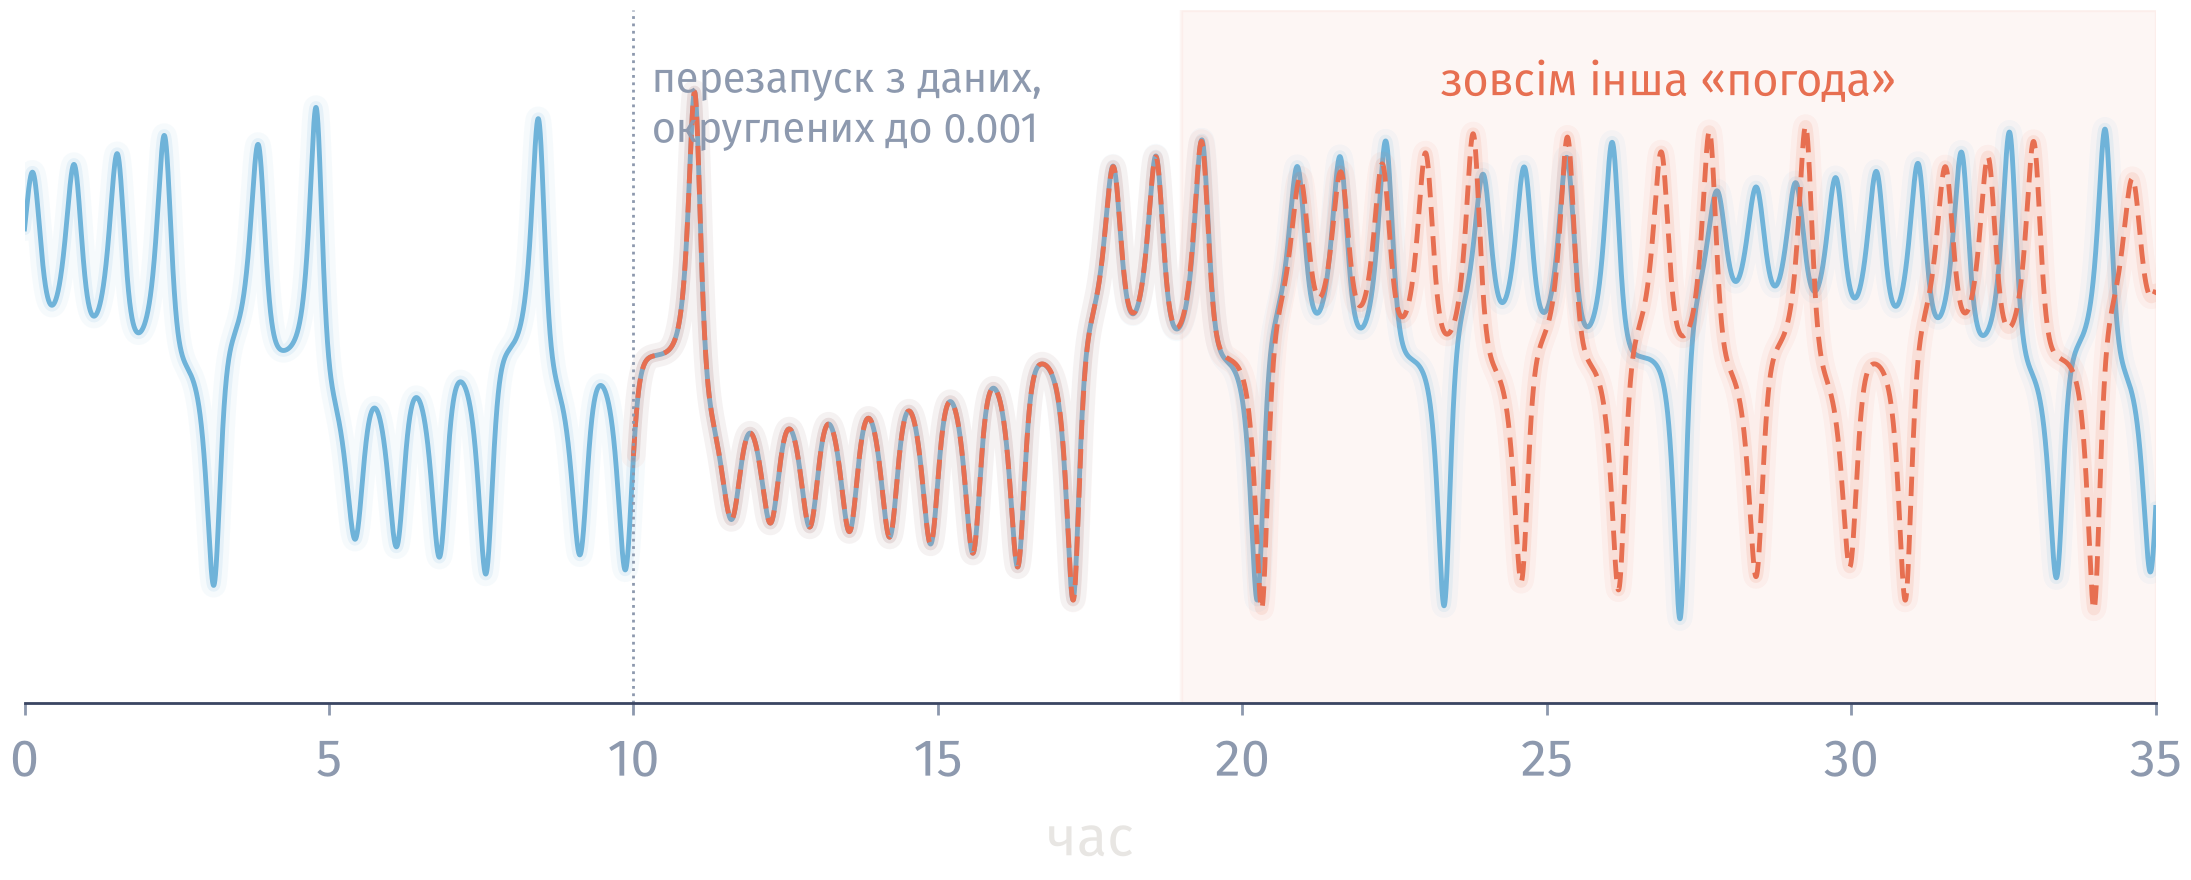
\includegraphics[height=0.5\textheight]{pop_rounding.png}\par\vspace{0.4em}
  \begin{columns}[c]
    \begin{column}{0.36\textwidth}
      \centering{\fontsize{16}{19}\selectfont\bfseries\color{NGold}0.506127 $\to$ 0.506}\\[0.2em]
      {\footnotesize\color{NDim}одне й те саме число, лише коротше}
    \end{column}
    \begin{column}{0.6\textwidth}
      \small Щоб не рахувати все спочатку, Лоренц вписав числа з роздруківки і пішов по каву.
      Повернувся, а в машині вже \gl{зовсім інша погода}. Комп'ютер не зламався: так поводяться самі рівняння.
      \\[0.2em]\dimtxt{\scriptsize На графіку наше відтворення цього досліду.}
    \end{column}
  \end{columns}
\end{frame}

% =====================================================================
% 3. МОДЕЛЬ
% =====================================================================
\begin{frame}{Конвекція та рівняння Лоренца}
  \begin{columns}[c]
    \begin{column}{0.47\textwidth}
      \centering
      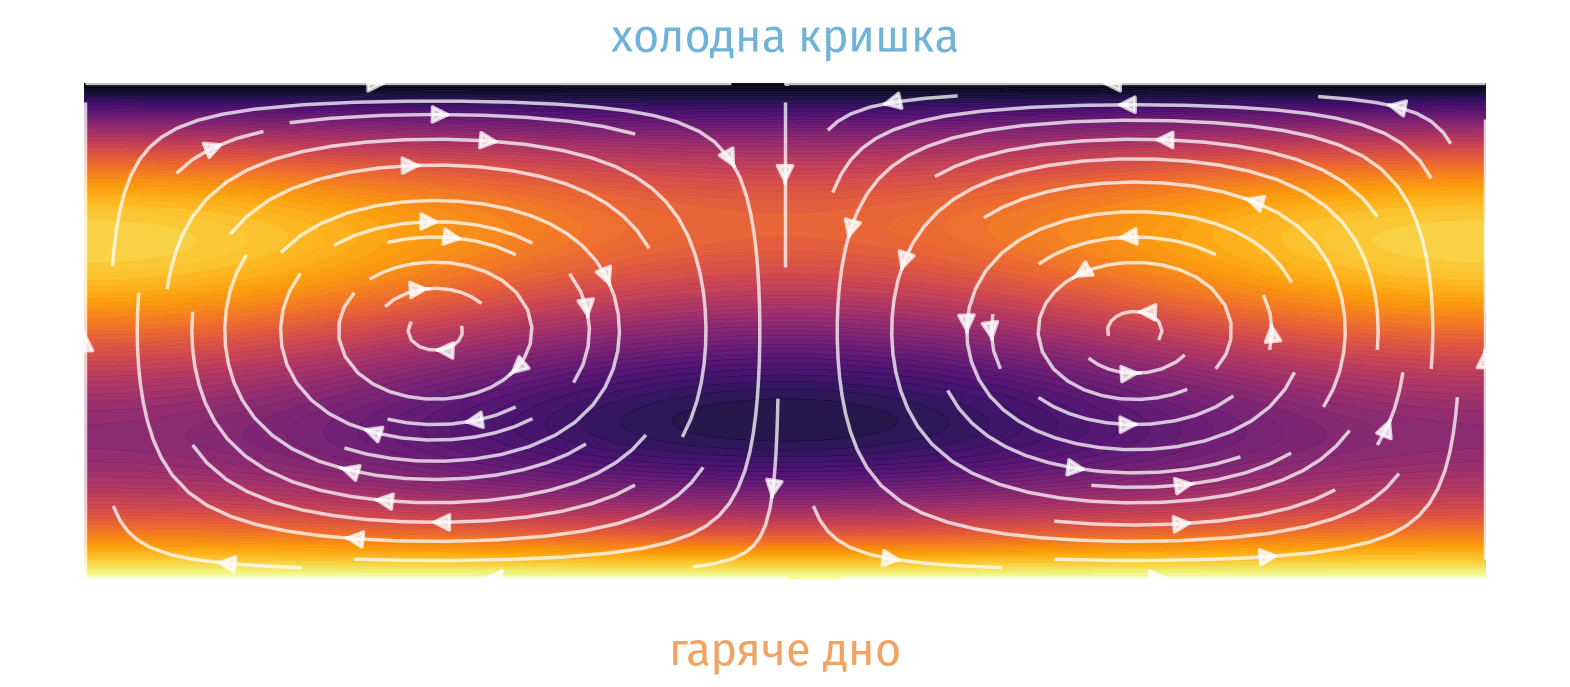
\includegraphics[width=\linewidth]{pop_convection.png}\\[0.6em]
      \small Знизу гаряче, зверху холодно. Тепла рідина піднімається, холодна опускається, і вона починає крутитися \gl{валами}.
    \end{column}
    \begin{column}{0.48\textwidth}
      \small Лоренц залишив від цієї картини лише три числа:
      \begin{bigeq}
        \vspace{-0.9em}
        \begin{align*}
          \dot x &= \sigma\,(y - x)\\
          \dot y &= x\,(r - z) - y\\
          \dot z &= x\,y - \beta z
        \end{align*}
        \vspace{-1.3em}
      \end{bigeq}
      \textcolor{NSky}{\bfseries $x$}\quad як швидко і в який бік крутиться вал\\[0.2em]
      \textcolor{NSky}{\bfseries $y$}\quad різниця тепла між потоками\\[0.2em]
      \textcolor{NSky}{\bfseries $z$}\quad як змінюється температура з висотою\\[0.2em]
      \textcolor{NGold}{\bfseries $r$}\quad як сильно гріємо
      \\[0.6em]\dimtxt{\footnotesize Класичні значення: $\sigma=10$, $\beta=\tfrac83$, $r=28$.}
    \end{column}
  \end{columns}
\end{frame}

% =====================================================================
% 4. ДЕТЕРМІНІЗМ VS ПЕРЕДБАЧУВАНІСТЬ
% =====================================================================
\begin{frame}[c]{Детермінізм і передбачуваність}
  \begin{columns}[T]
    \begin{column}{0.47\textwidth}
      \begin{card}[NSky]{Що нам гарантовано}
        Один старт веде до \textbf{одного} майбутнього:
        \[ \mathbf{x}(t) = \varphi^t(\mathbf{x}_0). \]
        Якби ми знали старт абсолютно точно, знали б усе наперед.
      \end{card}
    \end{column}
    \begin{column}{0.47\textwidth}
      \begin{card}[NOrange]{Що йде не так}
        Абсолютно точно не виміряти нічого. А два майже однакові старти з часом ведуть у \textbf{зовсім різні} боки.
        \[ \mathbf{x}_0 \approx \mathbf{y}_0, \quad\text{але}\quad \varphi^t\mathbf{x}_0 \not\approx \varphi^t\mathbf{y}_0 . \]
      \end{card}
    \end{column}
  \end{columns}
  \vspace{1.8em}
  \centering\large Це і є \gl{детермінований хаос}: правила точні, рух обмежений,\\ а дрібна похибка виростає у велику.
\end{frame}

% =====================================================================
% 5. СТИСКАННЯ І РОЗТЯГ
% =====================================================================
\begin{frame}{Що стається з близькими станами}
  \centering
  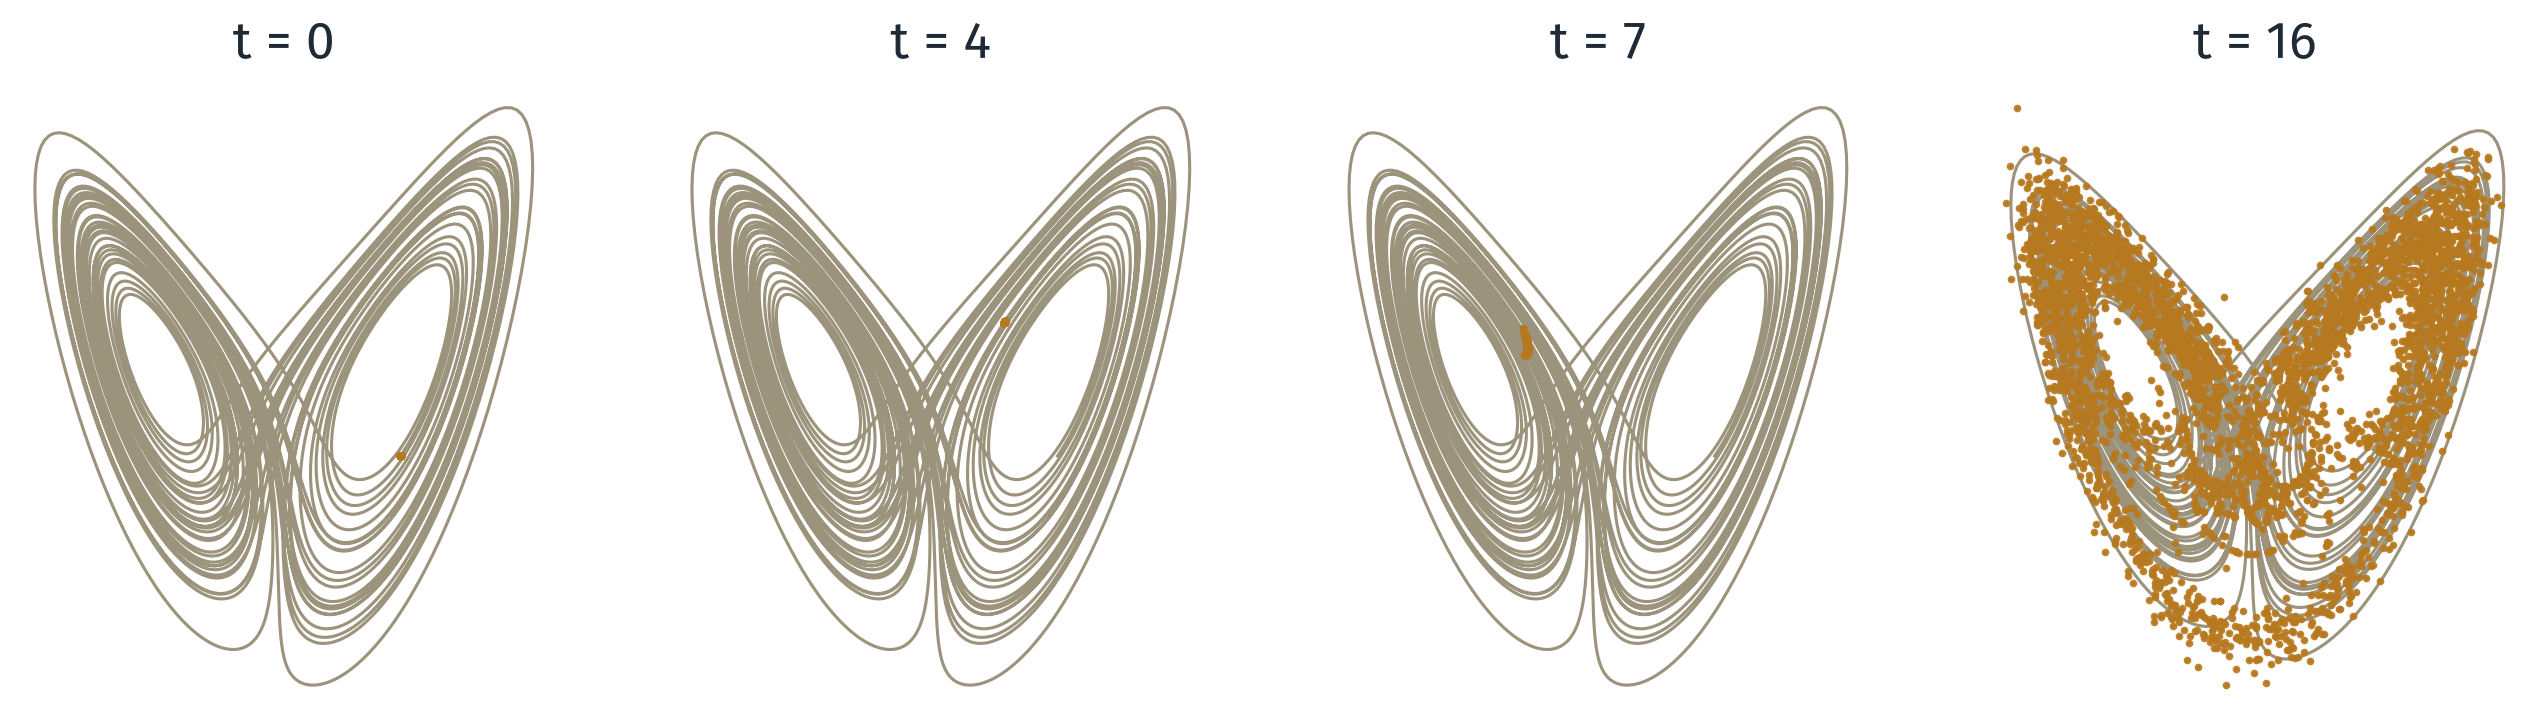
\includegraphics[height=0.42\textheight]{pop_blob.png}\\[0.8em]
  \normalsize Беремо 4000 майже однакових станів. Хмарка \gl{розтягується}, \gl{складається}\\
  і розходиться по всьому «метелику».
  \\[0.9em]
  \small При цьому її об'єм тане, приблизно в мільйон разів за одиницю часу:
  \[ \Div f = -(\sigma+1+\beta), \qquad V(t) = V_0\, e^{-13.67\,t}. \]
\end{frame}

% =====================================================================
% 6. ДИВНИЙ АТРАКТОР
% =====================================================================
\begin{frame}{Атрактор Лоренца}
  \begin{columns}[c]
    \begin{column}{0.52\textwidth}
      \centering
      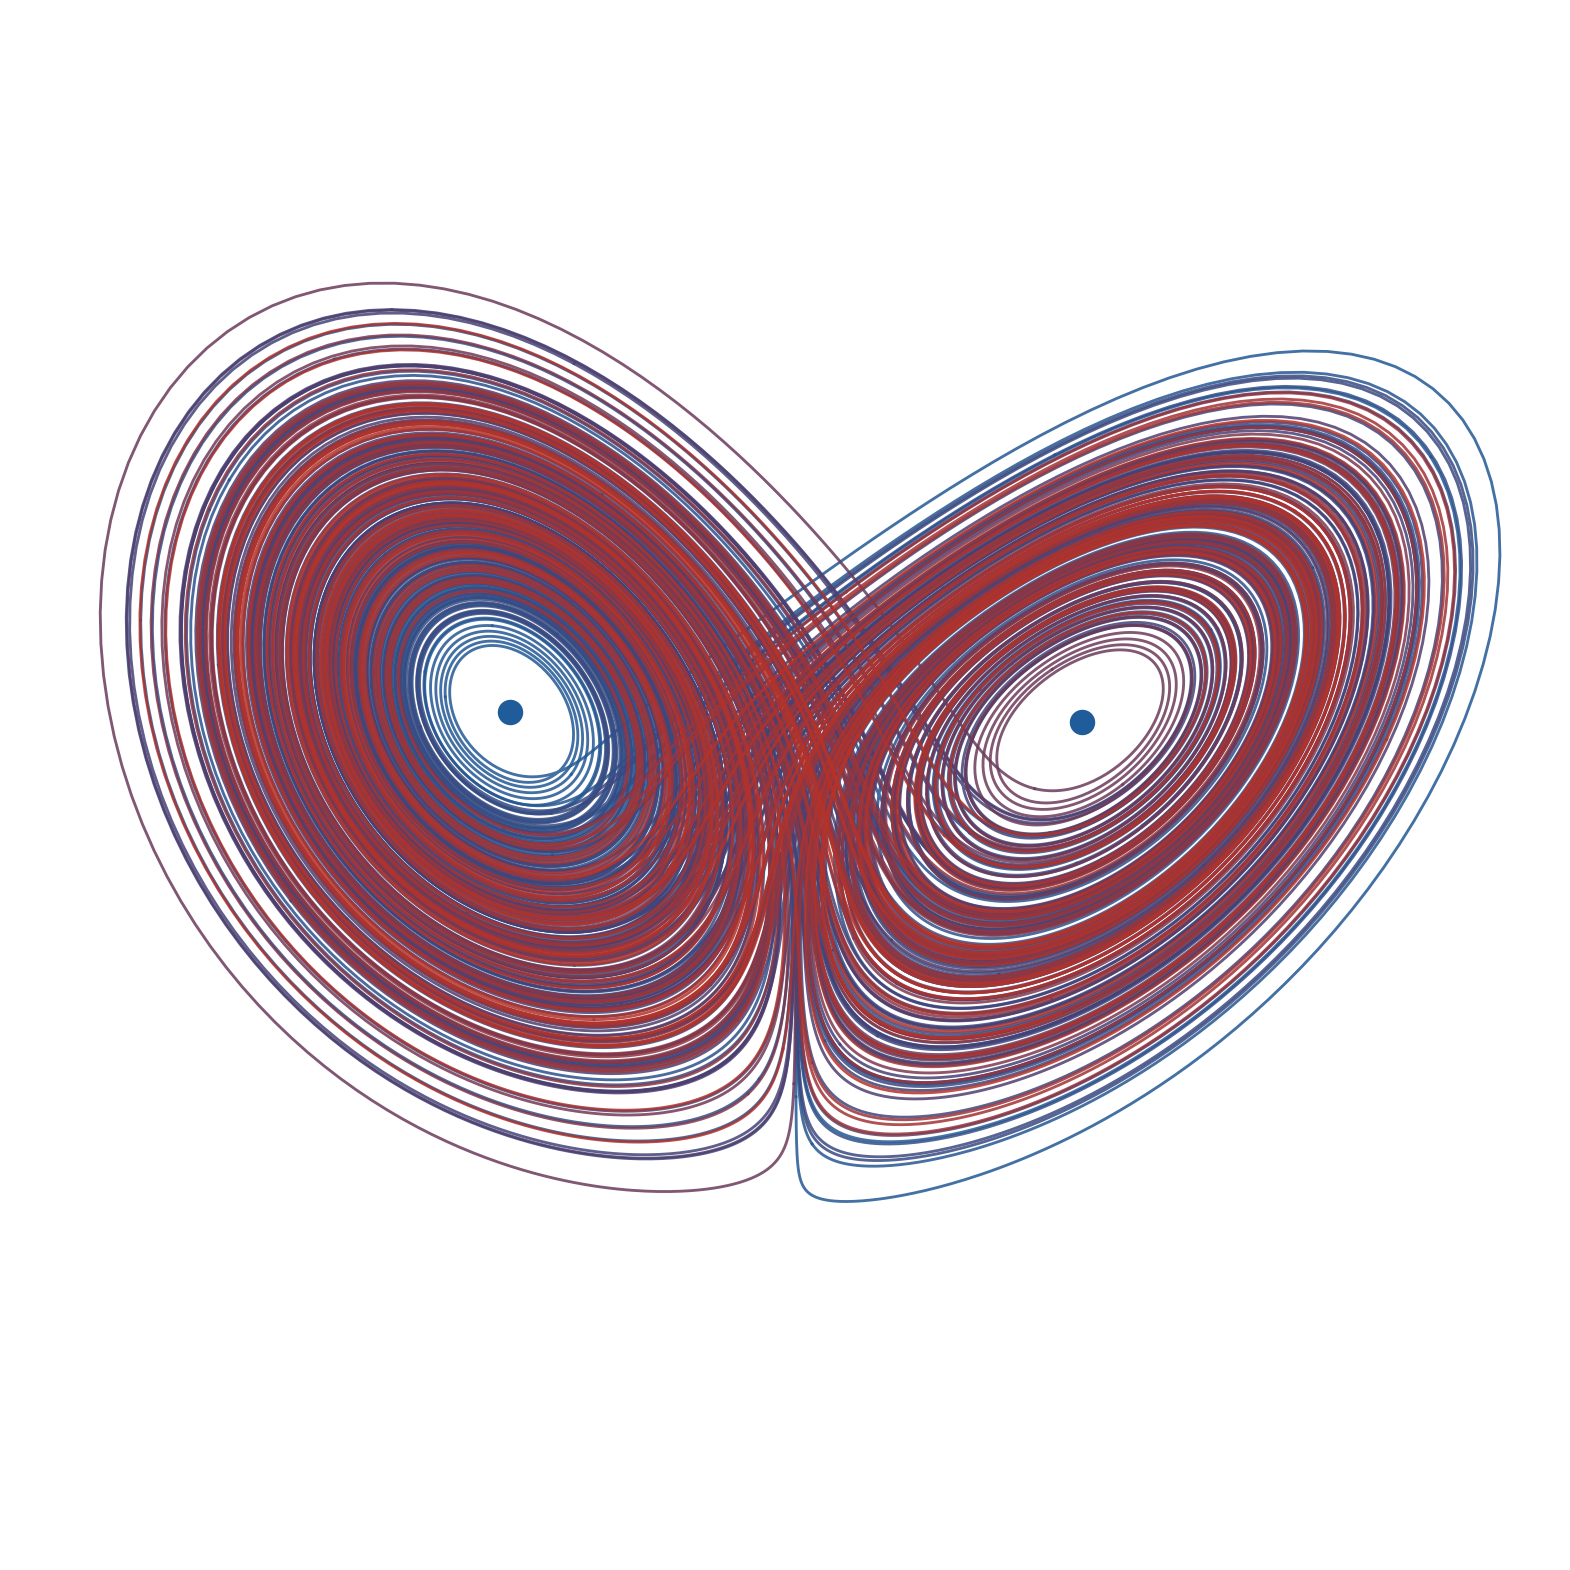
\includegraphics[height=0.76\textheight]{pop_attractor.png}
    \end{column}
    \begin{column}{0.44\textwidth}
      \large Звідки б ми не почали, траєкторія прийде сюди.\\[1em]
      \small \gl{Втекти вона не може:} далеко від центра рівняння завжди повертають її назад.\\[0.8em]
      \gl{Це не лінія і не поверхня:} її розмірність приблизно $\DKY$. Безліч тонких «листків», один над одним.\\[1.2em]
      \dimtxt{\footnotesize Що атрактор справді «дивний», строго довів В.~Такер у 2002 році.}
    \end{column}
  \end{columns}
\end{frame}

% =====================================================================
% 7. ШЛЯХ ДО ХАОСУ
% =====================================================================
\begin{frame}{Як змінюється рух зі зростанням $r$}
  \centering
  \begin{tikzpicture}[x=0.43cm]
    \shade[left color=NSky,right color=NOrange] (0,-0.05) rectangle (31,0.05);
    \draw[-{Latex[length=2mm]},NOrange,thick] (30.5,0) -- (31.6,0) node[right,font=\small]{$r$};
    \foreach \x/\col in {1/NSky, 13.93/NTeal, 24.06/NGold, 24.74/NOrange, 28/NInk}{
      \fill[\col] (\x,0) circle (0.11);
    }
    \node[above=3pt,font=\footnotesize,text=NSky,align=center] at (1,0) {\textbf{1}\\ з'являються вали};
    \node[above=3pt,font=\footnotesize,text=NTeal,align=center] at (13.93,0) {\textbf{13.93}\\ перші нерегулярні орбіти};
    \node[above=3pt,font=\footnotesize,text=NGold,align=center] at (22.6,0) {\textbf{24.06}\\ народжується метелик};
    \node[below=3pt,font=\footnotesize,text=NOrange,align=center] at (24.74,0) {\textbf{24.74}\\ рівний рух стає нестійким};
    \node[above=3pt,font=\footnotesize,text=NInk,align=center] at (29.2,0) {\textbf{28}\\ класика};
    \node[below=3pt,font=\footnotesize,text=NDim,align=center] at (7,0) {вали крутяться рівно};
  \end{tikzpicture}\\[0.3em]
  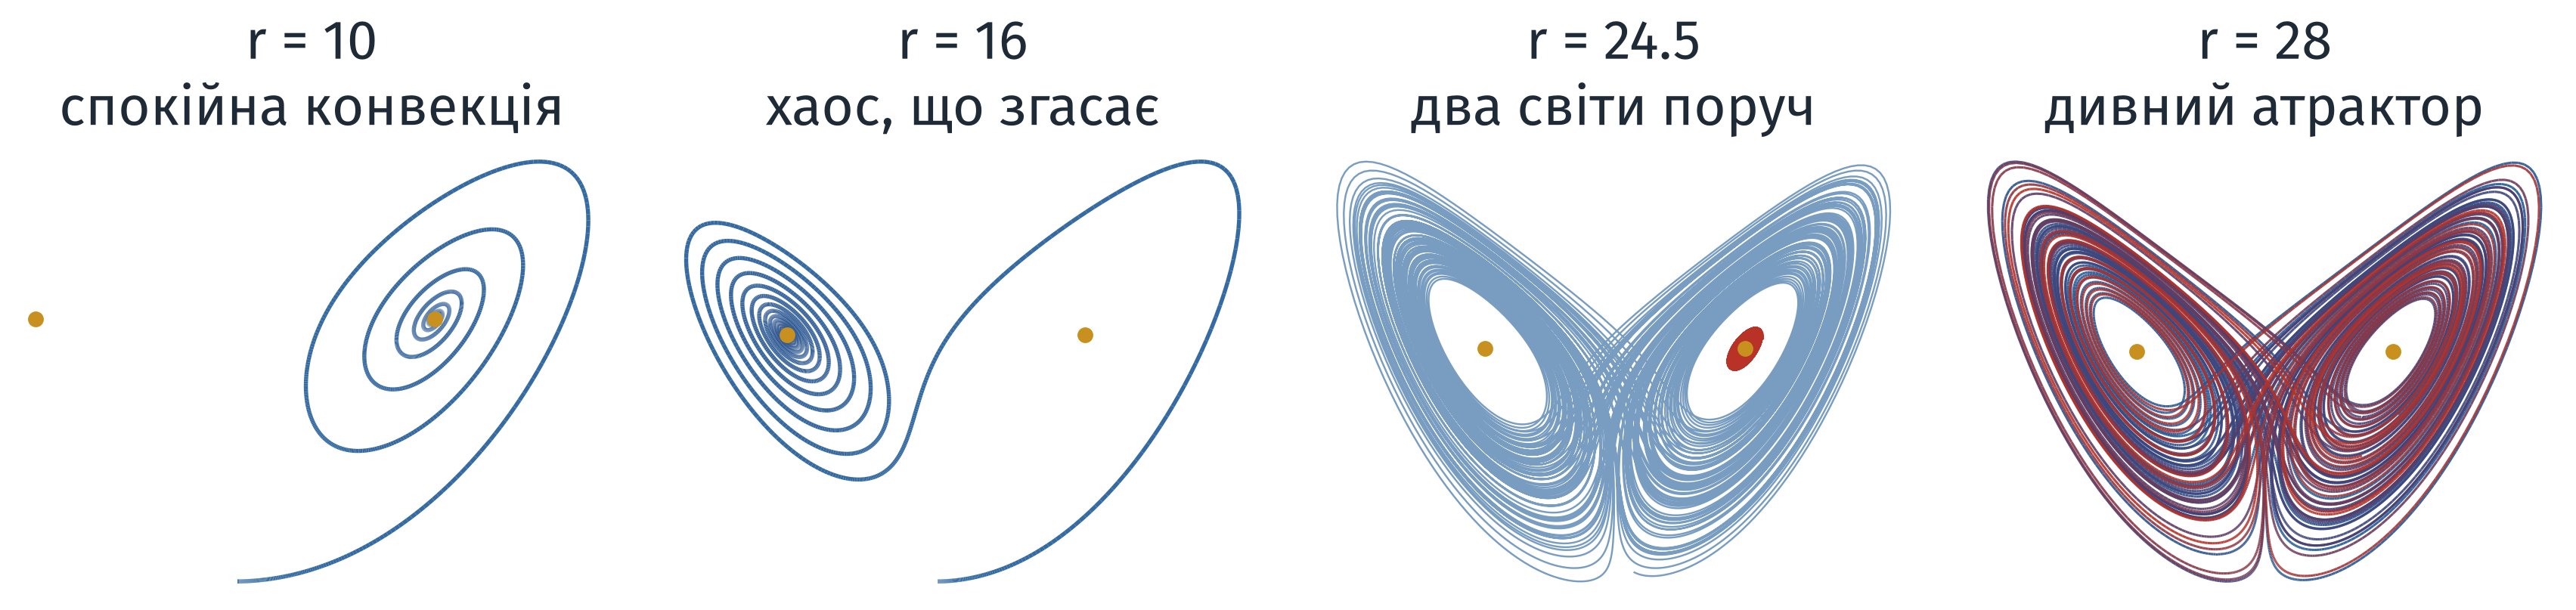
\includegraphics[width=\textwidth]{pop_gallery.png}\\[0.3em]
  \footnotesize\dimtxt{Поріг $24.74=\tfrac{470}{19}$ виведено аналітично, а $13.93$ і $24.06$ ми отримали чисельно.}
\end{frame}

% =====================================================================
% 8. ЕФЕКТ МЕТЕЛИКА
% =====================================================================
\begin{frame}{Чутливість до початкових умов}
  \begin{columns}[c]
    \begin{column}{0.6\textwidth}
      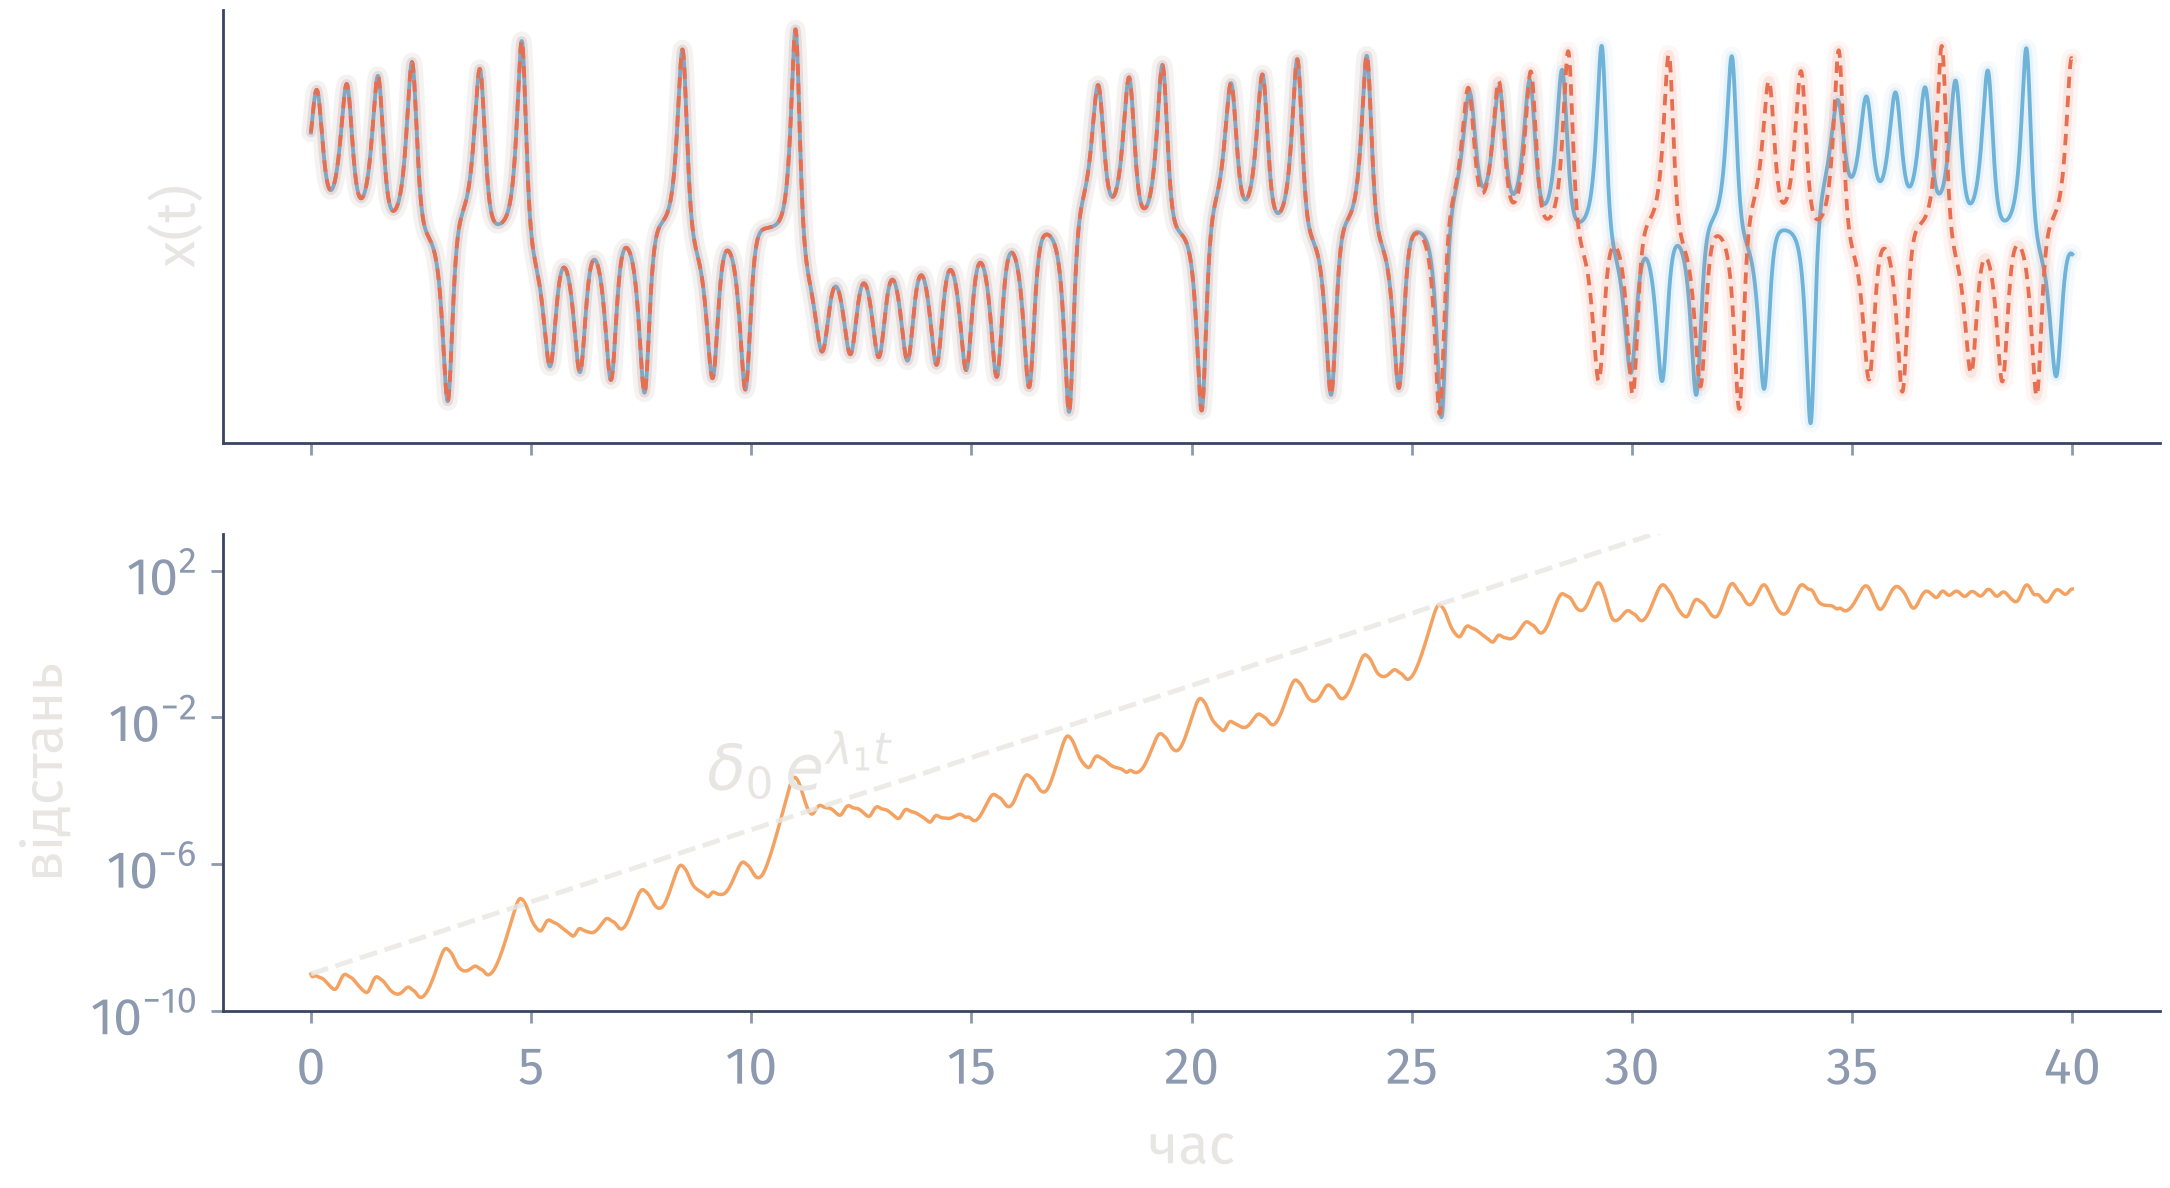
\includegraphics[width=\linewidth]{pop_butterfly.png}
    \end{column}
    \begin{column}{0.37\textwidth}
      \small Два прогнози відрізняються на $10^{-9}$. Спочатку їх не розрізнити, а потім вони живуть кожен своїм життям.
      \begin{bigeq}
        \Large $\delta(t) \approx \delta_0\, e^{\lambda_1 t}$
      \end{bigeq}
      \vspace{0.4em}
      Різниця \gl{подвоюється} кожні $\approx 0.77$ одиниці часу. Знову і знову.
    \end{column}
  \end{columns}
\end{frame}

% =====================================================================
% 9. ПОКАЗНИКИ ЛЯПУНОВА
% =====================================================================
\begin{frame}{Показники Ляпунова}
  \begin{columns}[c]
    \begin{column}{0.52\textwidth}
      \centering
      \begin{tikzpicture}
        \shade[ball color=NSky!70!NCard] (0,0) circle (0.75);
        \node[below=0.85cm,font=\footnotesize,text=NDim] at (0,0) {кулька станів};
        \draw[-{Latex[length=2.5mm]},NDim,thick] (1.05,0) -- node[above,font=\small,text=NInk]{час} (2.15,0);
        \begin{scope}[shift={(4.3,0)},rotate=18]
          \shade[ball color=NOrange!80!NCard] (0,0) ellipse (1.95 and 0.16);
        \end{scope}
        \node[font=\footnotesize,text=NDim] at (4.4,-1.15) {витягнута «голка»};
      \end{tikzpicture}
      \\[1em]
      \small Дивимося, як швидко кулька витягується в одних напрямках і сплющується в інших. Ці швидкості й називають показниками Ляпунова.
      \\[0.6em]\footnotesize\dimtxt{Обчислено алгоритмом Бенеттіна, $T=10^4$.}
    \end{column}
    \begin{column}{0.42\textwidth}
      \begin{plaincard}\stat[NOrange]{$\lambda_1 = +\lamOne$}{розтягує: звідси хаос}\end{plaincard}
      \begin{plaincard}\stat[NSky]{$\lambda_2 \approx 0$}{уздовж руху нічого не росте}\end{plaincard}
      \begin{plaincard}\stat[NTeal]{$\lambda_3 = \lamThree$}{сильно стискає}\end{plaincard}
      \centering\footnotesize Перевірка: їхня сума \lamSum, як і передбачає теорія.
    \end{column}
  \end{columns}
\end{frame}

% =====================================================================
% 10. МЕЖА ПРОГНОЗУ
% =====================================================================
\begin{frame}{Горизонт прогнозу}
  \begin{columns}[c]
    \begin{column}{0.55\textwidth}
      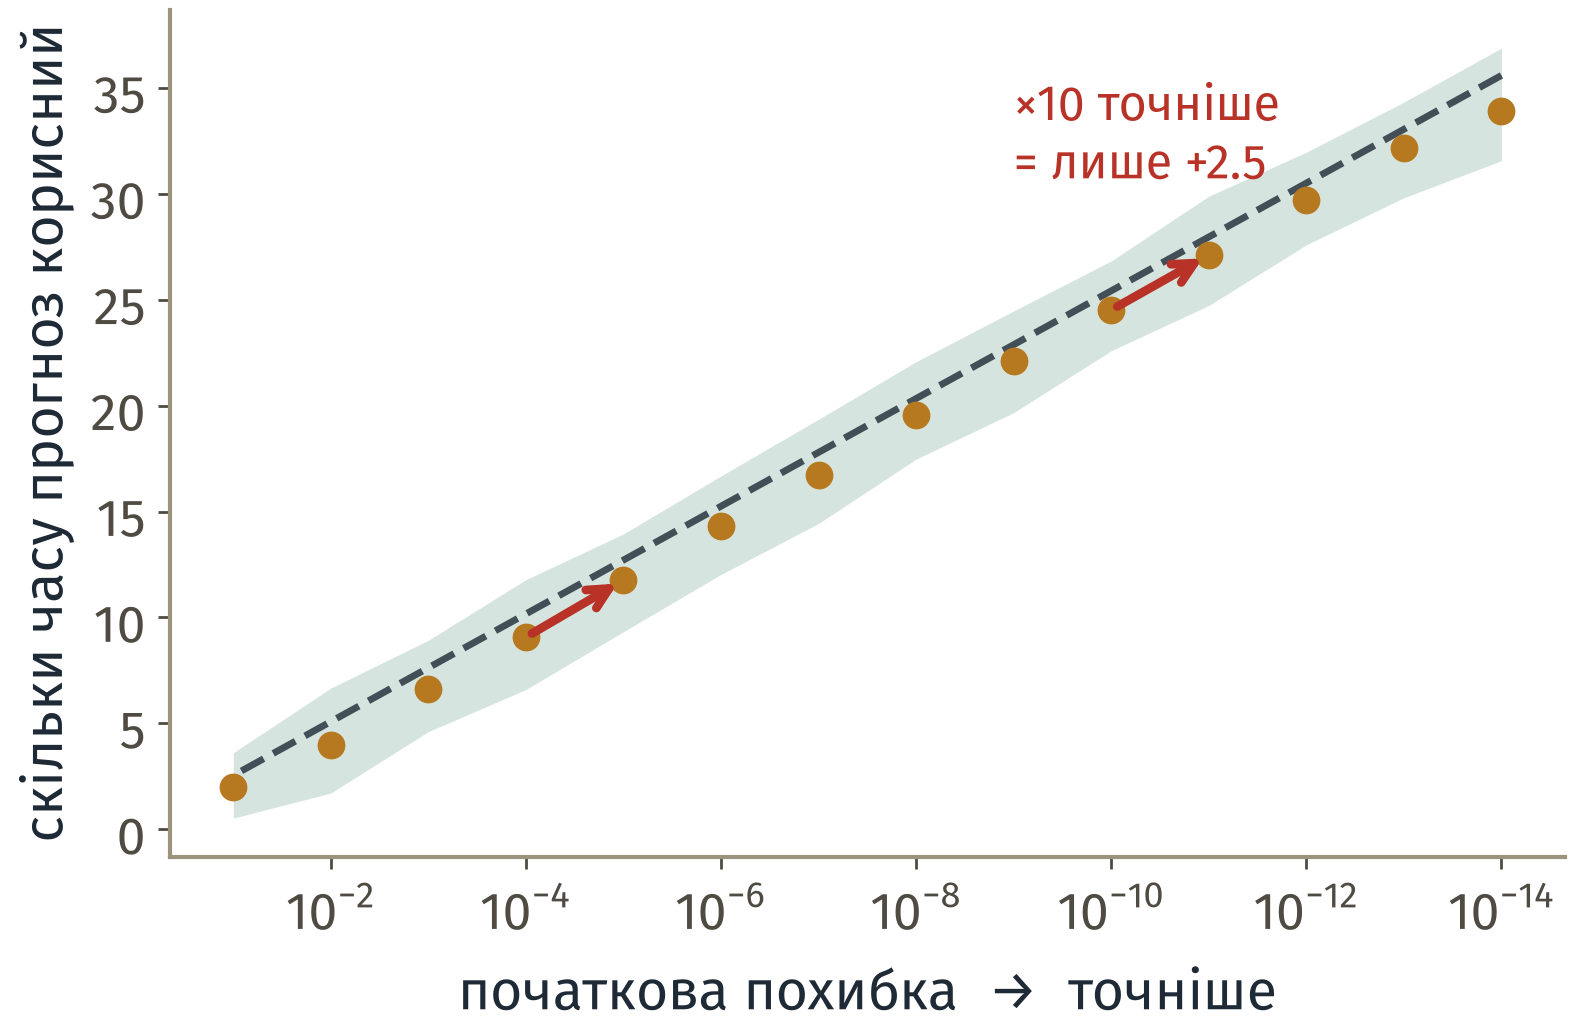
\includegraphics[width=\linewidth]{pop_horizon.png}
    \end{column}
    \begin{column}{0.42\textwidth}
      \small Виміряли в 10 разів точніше, а виграли лише
      \\[0.4em]
      \stat{$+\predGain$}{одиниці модельного часу}
      \\[0.6em]
      \begin{bigeq}
        $\displaystyle T_p \approx \frac{1}{\lambda_1}\ln\frac{\Delta}{\delta_0}$
      \end{bigeq}
      Точність стоїть під логарифмом, тому кожен наступний крок дається дедалі дорожче.\\[0.6em]
      \dimtxt{\footnotesize Для справжньої атмосфери межу оцінюють приблизно у два тижні.}
    \end{column}
  \end{columns}
\end{frame}

% =====================================================================
% 11. АНСАМБЛІ
% =====================================================================
\begin{frame}{Ансамблевий прогноз}
  \begin{columns}[c]
    \begin{column}{0.6\textwidth}
      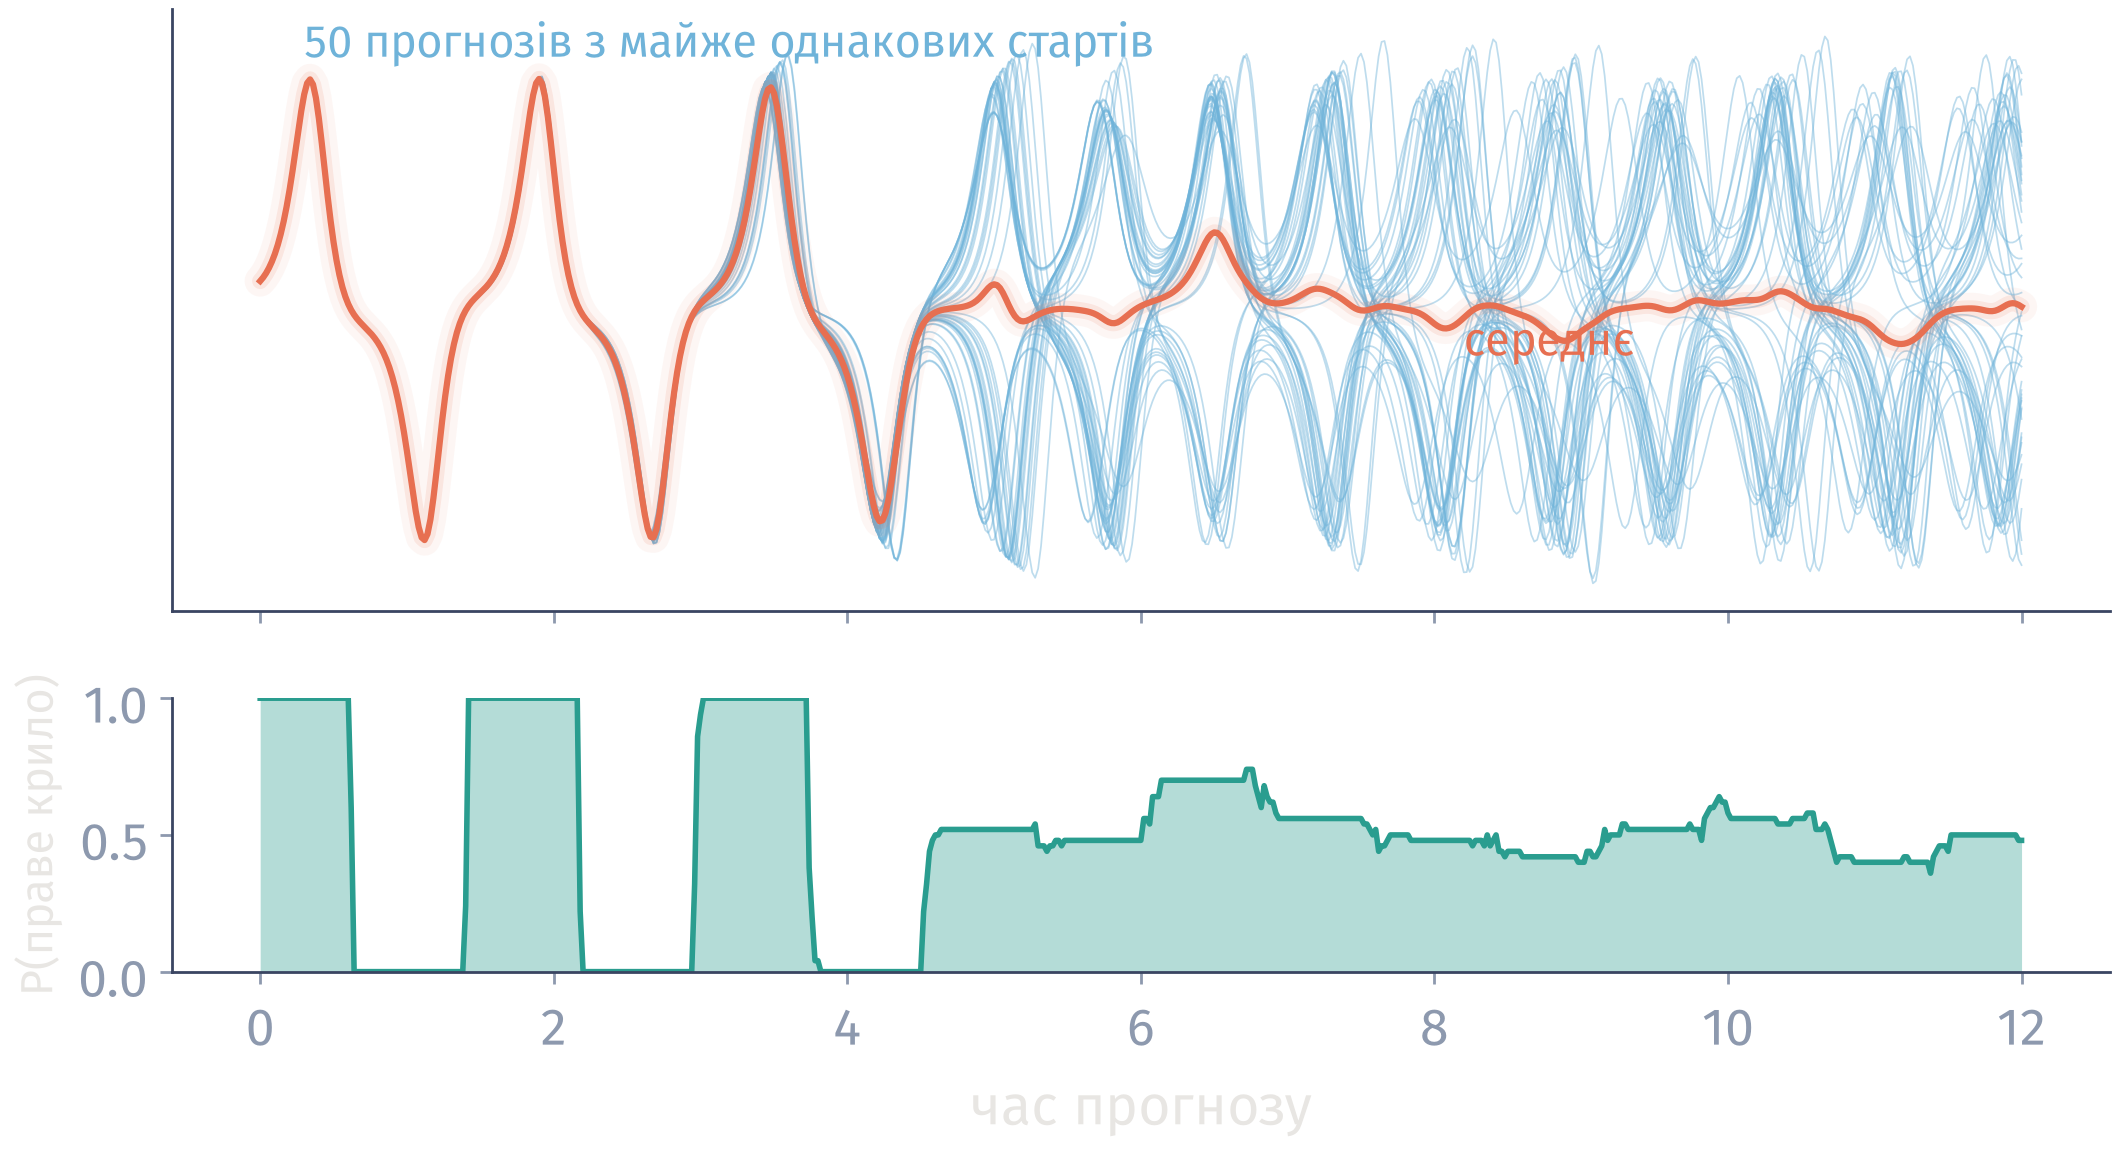
\includegraphics[width=\linewidth]{pop_ensemble.png}
    \end{column}
    \begin{column}{0.37\textwidth}
      \small Замість одного прогнозу запускають багато, щоразу з трохи іншого старту. Це \gl{ансамбль}.\\[0.9em]
      Якщо прогнози тримаються разом, їм можна довіряти. Якщо розбіглися віялом, ми \gl{не знаємо}, і це теж корисно знати.\\[0.9em]
      \dimtxt{\footnotesize Європейський центр прогнозів (ECMWF) двічі на добу запускає 51 такий варіант.}
    \end{column}
  \end{columns}
\end{frame}

% =====================================================================
% 12. АСИМІЛЯЦІЯ ДАНИХ
% =====================================================================
\begin{frame}{Асиміляція даних}
  \centering
  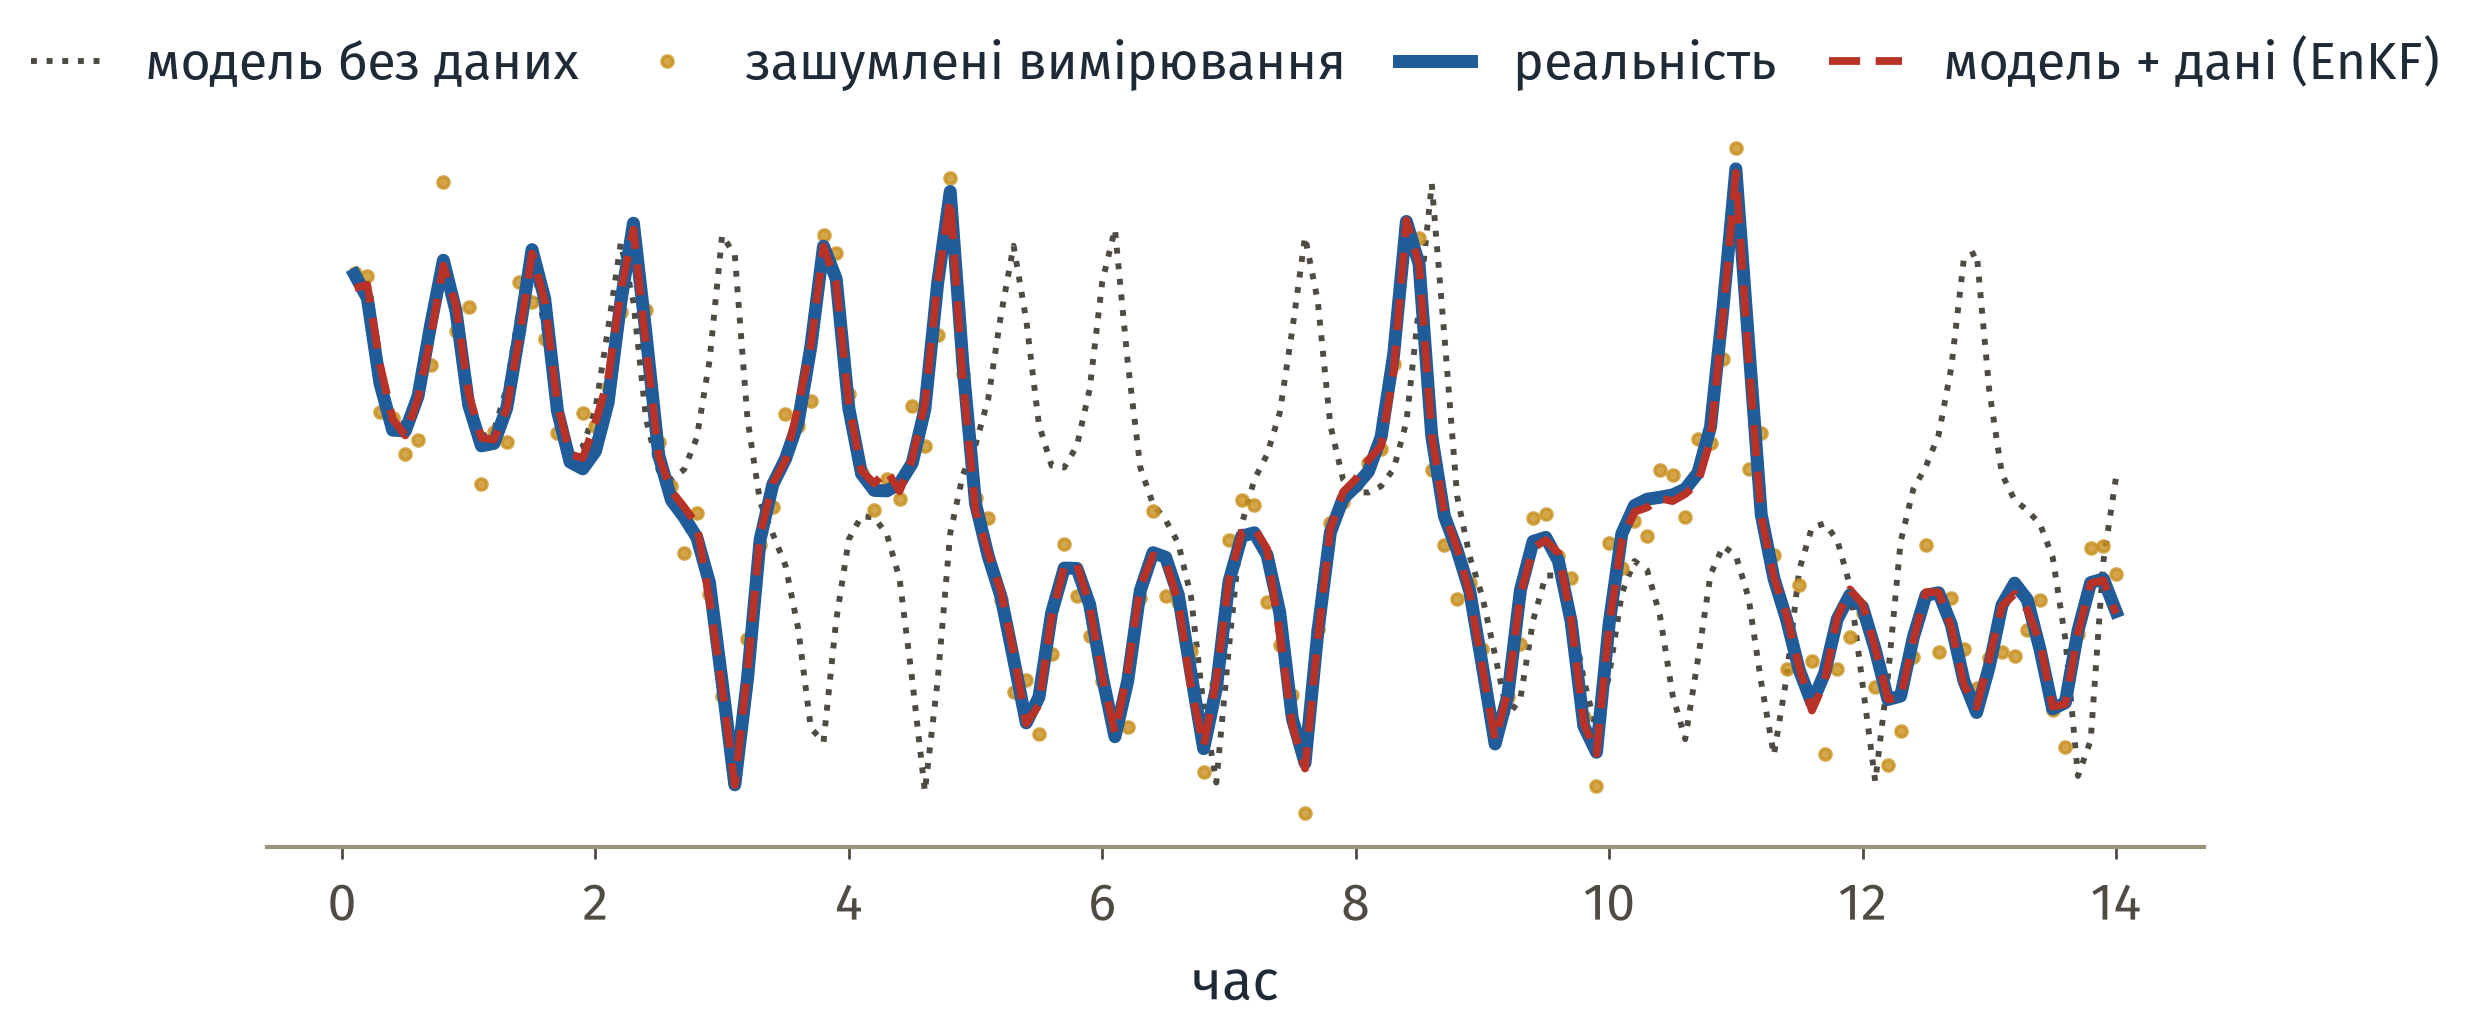
\includegraphics[height=0.42\textheight]{pop_enkf.png}\\[0.4em]
  \begin{columns}[c]
    \begin{column}{0.46\textwidth}
      \small Як навігатор: є розрахунок, де ми мали б бути, і є неточний сигнал GPS. Довіряємо кожному настільки, наскільки він надійний.
      \begin{bigeq}
        $\mathbf{x}^{a} = \mathbf{x}^{f} + K\big(\mathbf{y} - H\mathbf{x}^{f}\big)$
      \end{bigeq}
    \end{column}
    \begin{column}{0.5\textwidth}
      \footnotesize\centering Середня похибка в нашому досліді (фільтр EnKF):\\[0.5em]
      \begin{columns}[T]
        \begin{column}{0.33\linewidth}\stat[NDim]{\enkfFree}{модель сама}\end{column}
        \begin{column}{0.33\linewidth}\stat[NSand]{2.0}{шум вимірів}\end{column}
        \begin{column}{0.33\linewidth}\stat[NOrange]{\enkfRmse}{разом}\end{column}
      \end{columns}
    \end{column}
  \end{columns}
\end{frame}

% =====================================================================
% 13. ВЛАСНІ РЕЗУЛЬТАТИ
% =====================================================================
\begin{frame}[c]{Перевірка результатів}
  \centering\small
  \renewcommand{\arraystretch}{1.45}
  \begin{tabular}{lcc}
    \textcolor{NDim}{що рахувалося} & \textcolor{NDim}{у нас} & \textcolor{NDim}{у літературі}\\
    найбільший показник Ляпунова & \gl{\lamOne} & 0.9056\\
    розмірність Каплана--Йорке & \gl{\DKY} & 2.06\\
    кореляційна розмірність & \gl{\DTwo} & 2.05\\
    поява перших нерегулярних орбіт, $r$ & \gl{\rHom} & 13.926\\
    народження атрактора, $r$ & \gl{\rAlo} & 24.06\\
  \end{tabular}
  \\[1.6em]
  \footnotesize\dimtxt{Код власний (Python + Numba), формули перевірено в SymPy, коректність коду перевіряють 11 тестів.}
\end{frame}

% =====================================================================
% 14. ВИСНОВКИ
% =====================================================================
\begin{frame}[c]{Висновки}
  \begin{columns}[T]
    \begin{column}{0.3\textwidth}
      {\large\bfseries\color{NOrange} Просте буває непередбачуваним}\\[0.6em]
      \small Вистачило трьох рівнянь.
    \end{column}
    \begin{column}{0.3\textwidth}
      {\large\bfseries\color{NGold} У хаосу є форма}\\[0.6em]
      \small Де саме буде точка, невідомо. Але вона на «метелику», і середні величини стійкі.
    \end{column}
    \begin{column}{0.3\textwidth}
      {\large\bfseries\color{NTeal} Прогнозувати все одно можна}\\[0.6em]
      \small Недалеко, з імовірностями і постійно звіряючись із даними.
    \end{column}
  \end{columns}
  \vspace{2.6em}
  \centering
  \bigquote{Хаос — це коли теперішнє визначає майбутнє, але наближене теперішнє не визначає наближено майбутнього}{Едвард Лоренц}
\end{frame}

% =====================================================================
% 15. ДЯКУЮ
% =====================================================================
{\setbeamertemplate{footline}{}
\setbeamertemplate{background canvas}{}
\begin{frame}[plain]
  \begin{tikzpicture}[remember picture,overlay]
    \fill[NNight] (current page.south west) rectangle (current page.north east);
    \node[opacity=0.55,inner sep=0] at (current page.center)
      {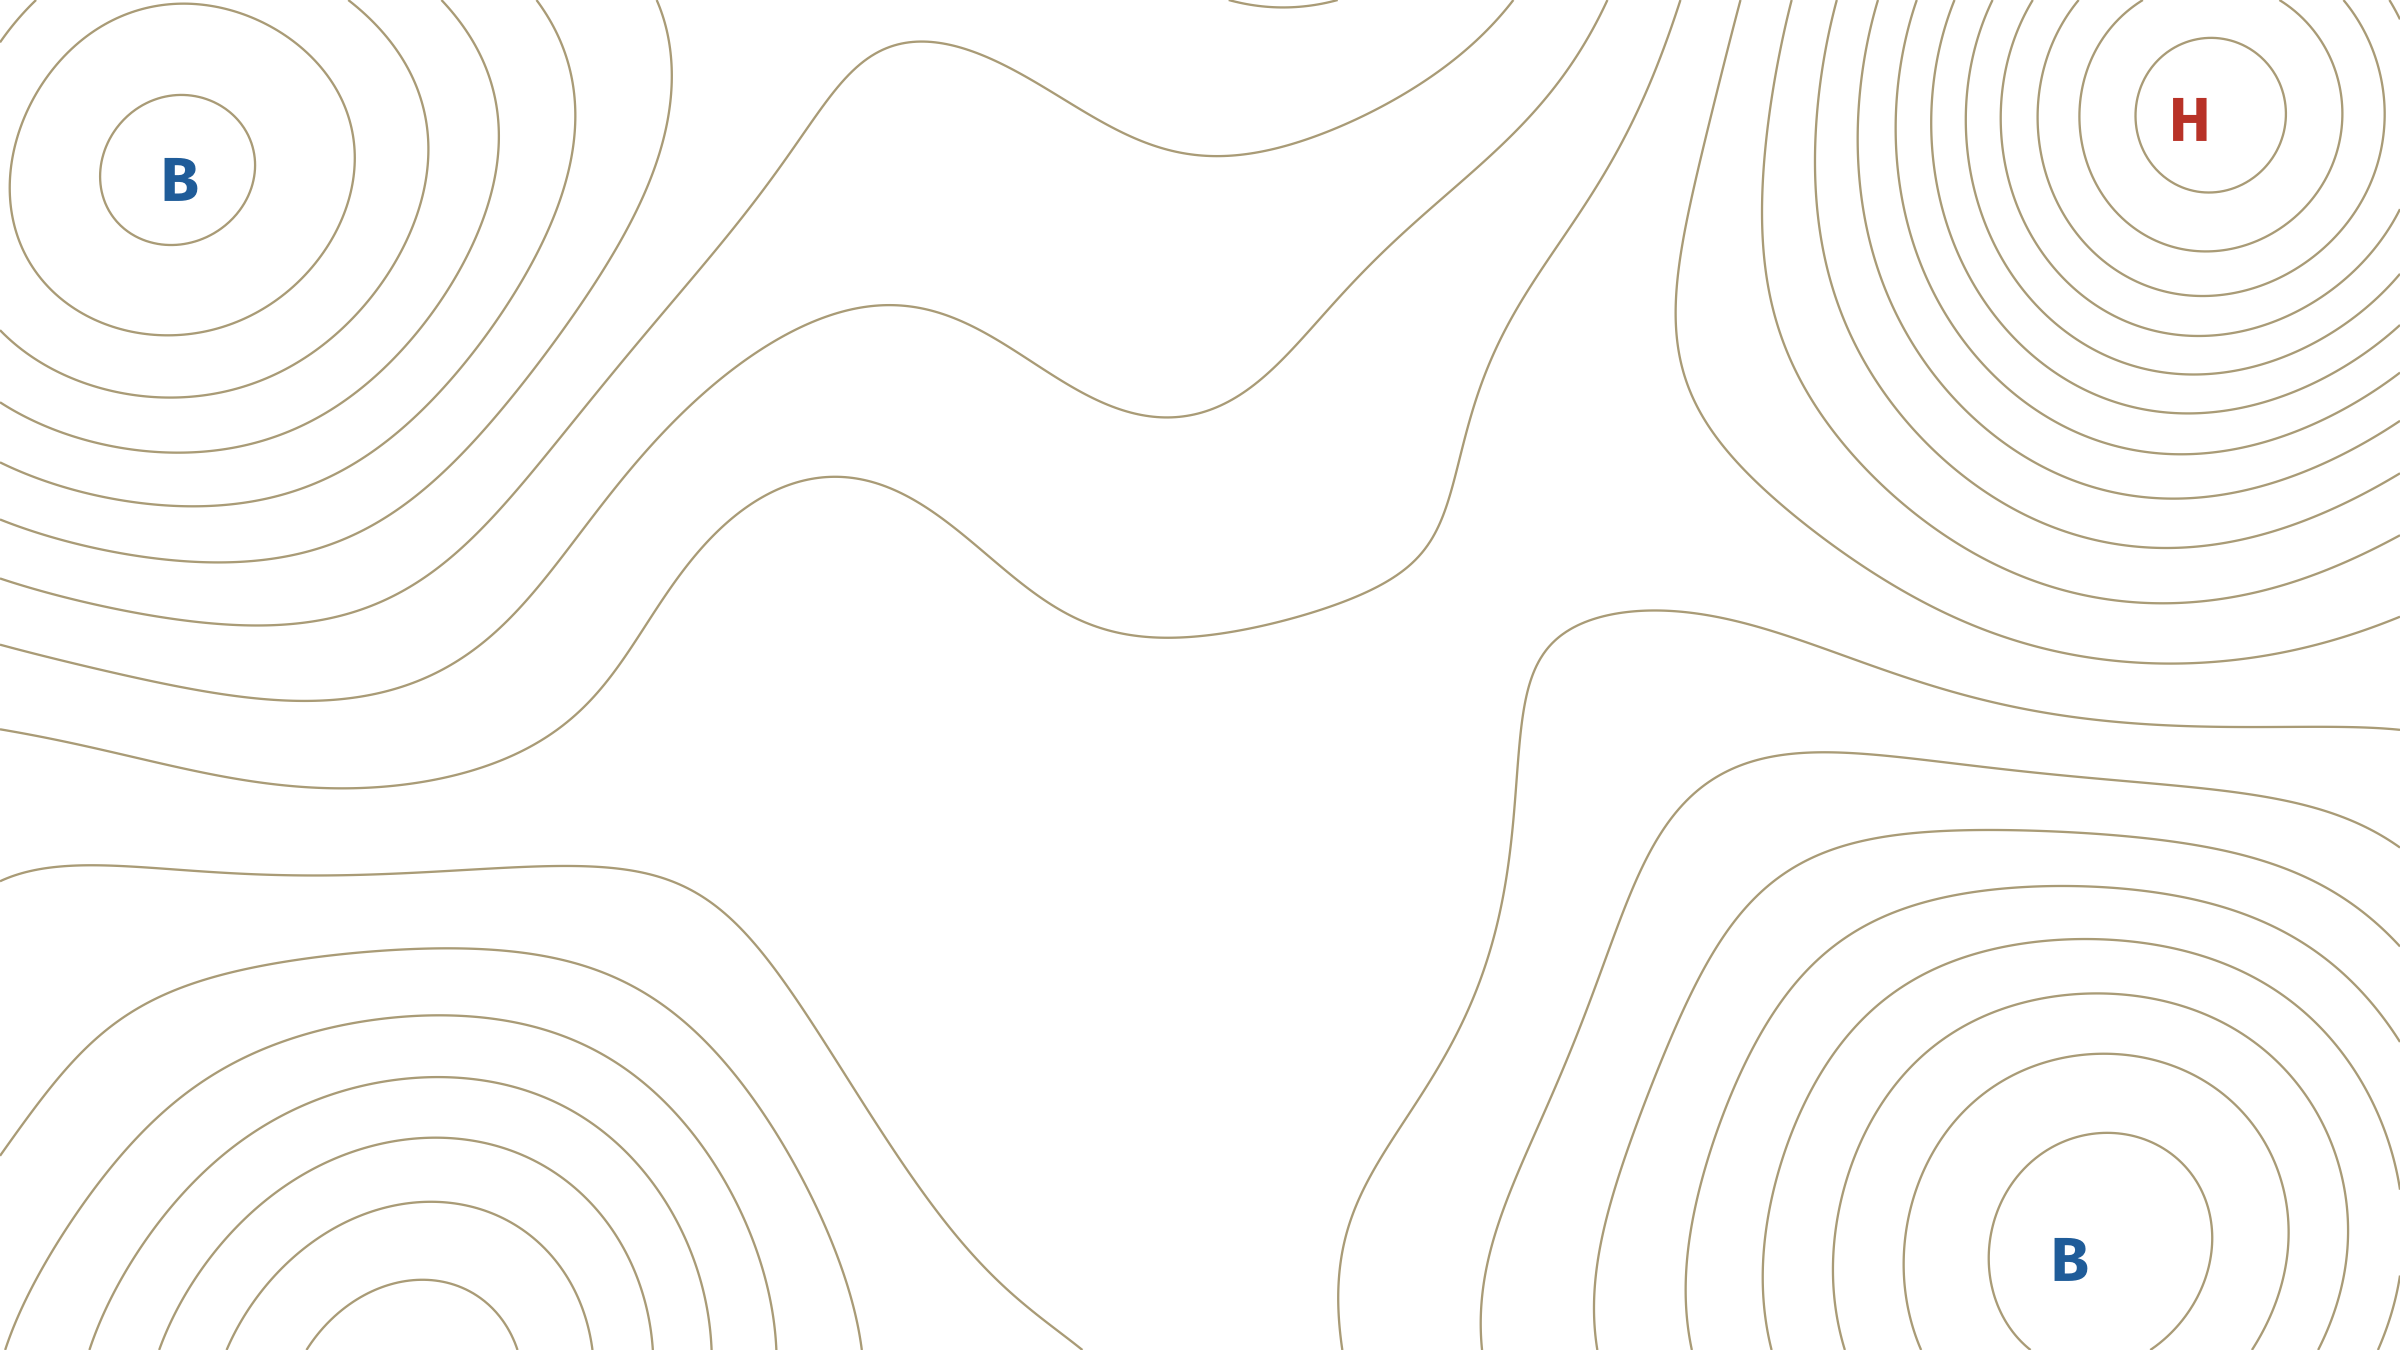
\includegraphics[width=\paperwidth,height=\paperheight]{pop_isobars_title.png}};
    \node[font=\fontsize{30}{34}\selectfont\bfseries,text=NInk] at ($(current page.center)+(0,0.45)$) {Дякую за увагу!};
    \node[inner sep=0] at ($(current page.center)+(0,-0.35)$) {\Nfront};
    \node[text=NDim,font=\large] at ($(current page.center)+(0,-1.05)$) {Запитання?};
  \end{tikzpicture}
\end{frame}}

% =====================================================================
% БОНУС: ЛОРЕНЦ ПОЗА ПОГОДОЮ (запасні слайди, experiments/applications.py)
% =====================================================================
\begin{frame}{Де ще зустрічаються ці рівняння}
  \begin{columns}[T]
    \begin{column}{0.48\textwidth}
      \begin{card}[NSky]{Фізика}
        \small
        \begin{itemize}
          \item[] \gl{Лазер} — одномодовий лазер точно зводиться до рівнянь Лоренца (Хакен, 1975)
          \item[] \gl{Динамо} — дисковий генератор хаотично міняє полярність, як поле Землі (Кноблох, 1981)
          \item[] \gl{Термосифон} — рідина в нагрітому кільці хаотично змінює напрям течії
          \item[] \gl{Водяне колесо} Малкуса (1972) — далі
        \end{itemize}
      \end{card}
    \end{column}
    \begin{column}{0.48\textwidth}
      \begin{card}[NOrange]{Техніка й дані}
        \small
        \begin{itemize}
          \item[] \gl{Електродвигуни} — безщітковий двигун може бути хаотичним «за Лоренцом» (Хематі, 1994)
          \item[] \gl{Секретний зв'язок} на хаотичних схемах (Куомо–Оппенгейм, 1993)
          \item[] \gl{Машинне навчання} — Лоренц-63 як еталонний тест для нейромереж
          \item[] \gl{Відкриття законів з даних} — SINDy (2016)
        \end{itemize}
      \end{card}
    \end{column}
  \end{columns}
  \vspace{0.2em}
  \centering\small\gl{Хаос — властивість рівнянь, а не атмосфери:} де з'являються ці рівняння, там з'являється метелик.
\end{frame}

\begin{frame}{Водяне колесо Малкуса}
  \centering
  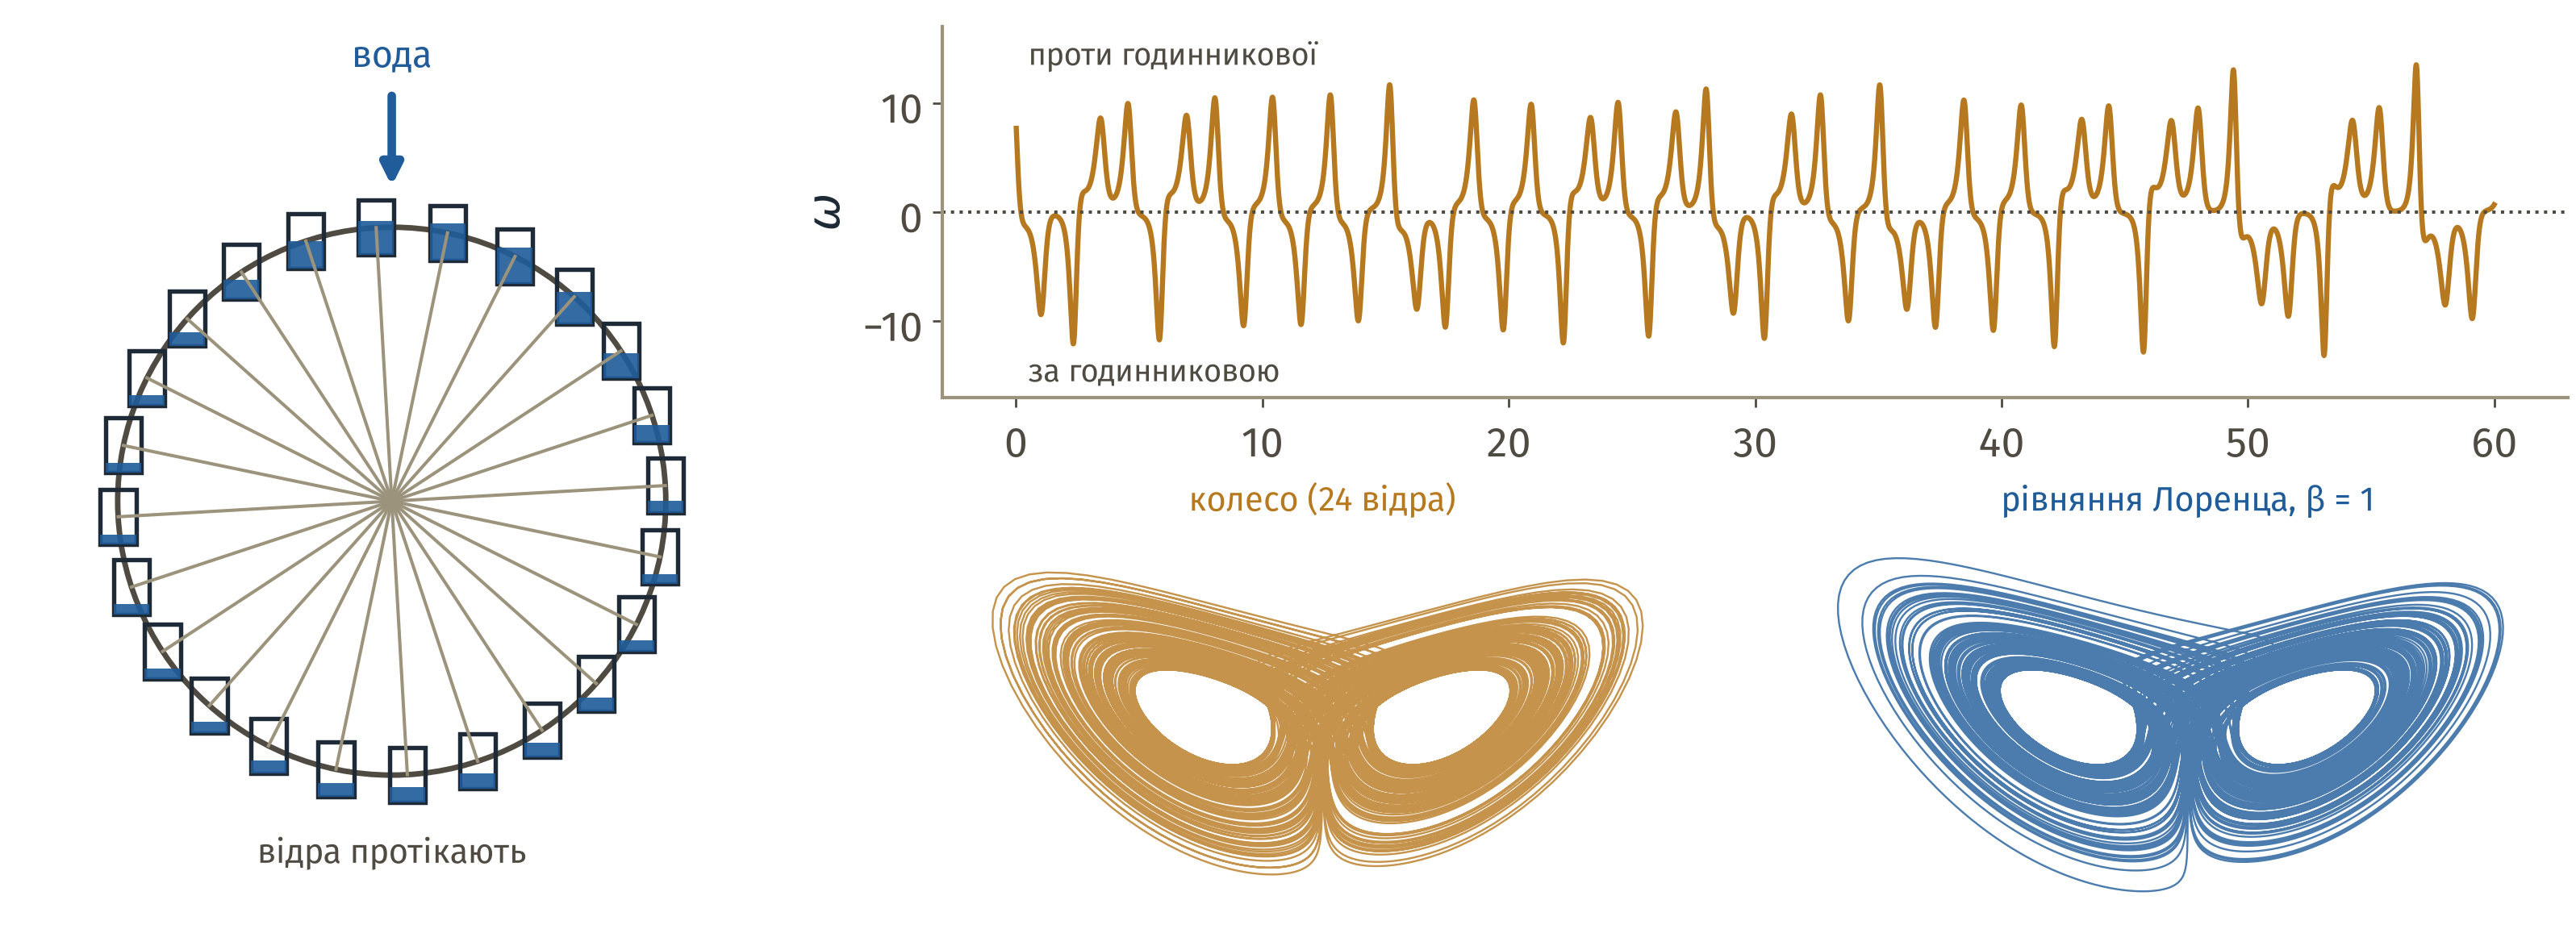
\includegraphics[height=0.46\textheight]{pop_wheel.png}\\[0.2em]
  \begin{columns}[T]
    \begin{column}{0.5\textwidth}
      \small Вода ллється у верхні відра, всі протікають. Важкий бік тягне колесо вниз; розігнавшись, воно не встигає наповнювати відра, гальмує\ldots\ і \hl{розвертається}: \wheelRev\ реверсів за 270 од. часу.
    \end{column}
    \begin{column}{0.46\textwidth}
      \begin{bigeq}
        \footnotesize $\omega\to x,\quad \sum m_i\sin\varphi_i\to y,\quad \sum m_i\cos\varphi_i\to z$
      \end{bigeq}
      \footnotesize Перші фур'є-моди маси дають \gl{точно Лоренца з $\beta=1$}: всі моди витікають з однаковою швидкістю. У нас вийшло: $\lambda_1=\wheelLam$, хаос при $r>r_H=\wheelHopf$.
    \end{column}
  \end{columns}
\end{frame}

\begin{frame}{Хаотичний зв'язок}
  \begin{columns}[c]
    \begin{column}{0.6\textwidth}
      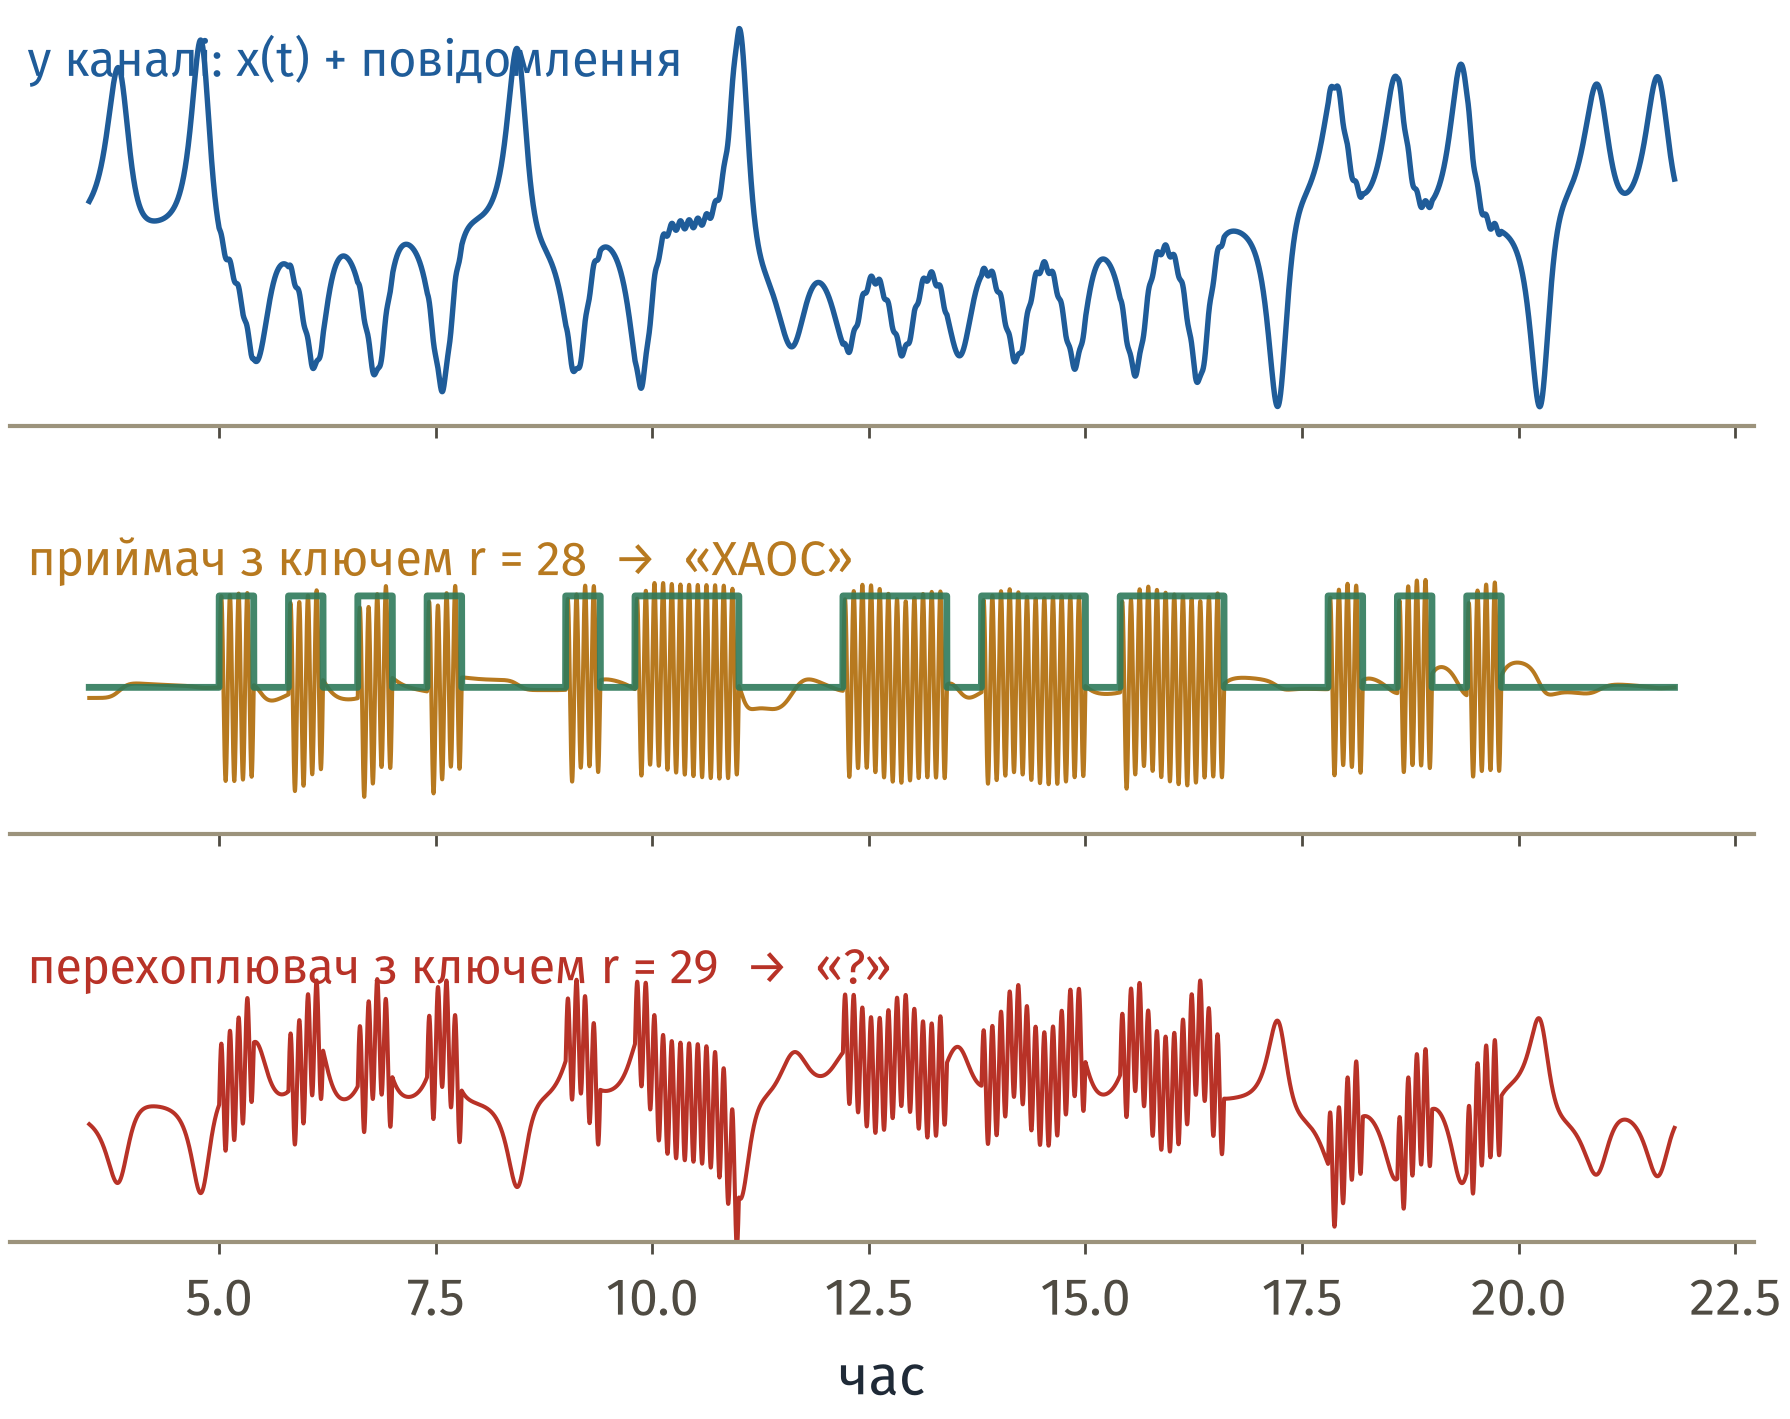
\includegraphics[width=\linewidth]{pop_secret.png}
    \end{column}
    \begin{column}{0.38\textwidth}
      \small Передавач додає до хаотичного $x(t)$ слабке повідомлення (\secPct\% сигналу) — азбукою Морзе «ХАОС».
      \begin{card}[NTeal]{Синхронізація}
        \footnotesize Приймач — копія системи, яку «веде» сигнал $s=x+m$. Похибка $(e_y,e_z)$ згасає, бо $\dot V = -e_y^2-\beta e_z^2<0$. Тоді $m \approx s - x_r$.
      \end{card}
      \begin{card}[NOrange]{Але це не криптографія}
        \footnotesize Перебір «ключів» $r'$ показав: повідомлення читається навіть при $r'=28+\secMaxOkDr$. Ключ угадують за кілька спроб — такі схеми зламано ще 1995 р. (Перес, Сердейра).
      \end{card}
    \end{column}
  \end{columns}
\end{frame}

\begin{frame}{Прогноз нейромережею}
  \centering
  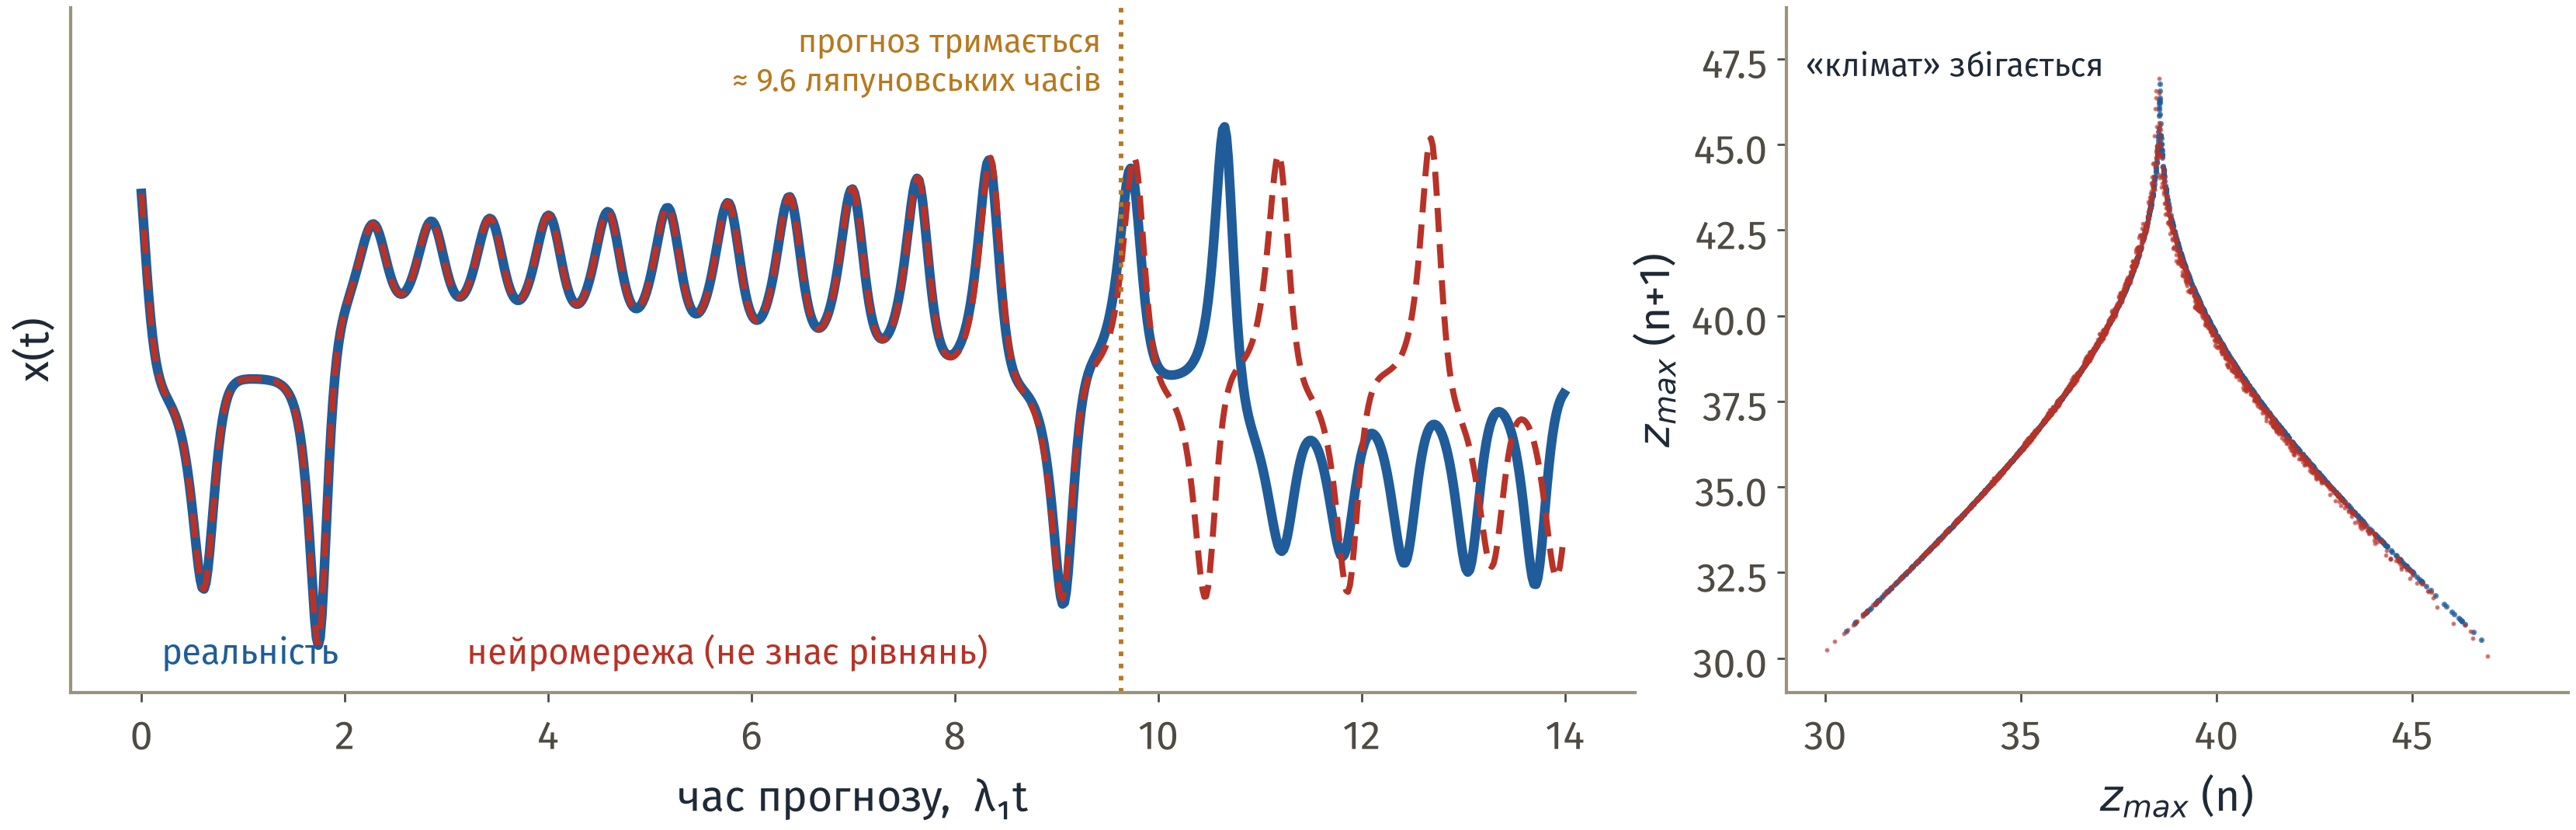
\includegraphics[height=0.44\textheight]{pop_reservoir.png}\\[0.1em]
  \begin{columns}[T]
    \begin{column}{0.5\textwidth}
      \small \gl{Мережа луни}: 800 випадково з'єднаних «нейронів» слухають ряд $x,y,z$; навчається лише вихідний шар (лінійна регресія). Далі мережа прогнозує сама, живлячись власним виходом.
    \end{column}
    \begin{column}{0.46\textwidth}
      \stat{\esnVT}{ляпуновських часів (середнє з 30 стартів: \esnVTmin–\esnVTmax)}
      \vspace{0.2em}
      \footnotesize Далі — розбіжність: \hl{метелика не обдуриш}. Але відображення $z_n\!\to z_{n+1}$ (праворуч) мережа відтворює: «погоду» забуває, «клімат» пам'ятає.
    \end{column}
  \end{columns}
\end{frame}

\begin{frame}{Відновлення рівнянь з даних}
  \begin{columns}[c]
    \begin{column}{0.47\textwidth}
      \small Даємо лише виміряні $x(t),y(t),z(t)$ і словник кандидатів $1,x,y,z,x^2,xy,\ldots,z^2$. Розріджена регресія викидає зайве (Брантон та ін., 2016):
      \begin{bigeq}
        \vspace{-0.8em}
        \begin{align*}
          \dot x &= -\sinSigma\,x + \sinSigma\,y\\
          \dot y &= \sinRho\,x - y - xz\\
          \dot z &= xy - \sinBeta\,z
        \end{align*}
        \vspace{-1.3em}
      \end{bigeq}
      \footnotesize З шумом $\pm0.5$ і згладжуванням: $\sigma=\sinNSigma$, $r=\sinNRho$, $\beta=\sinNBeta$.
      \begin{card}[NGold]{А тепер — колесо}
        \footnotesize Дані водяного колеса $\to$ SINDy знаходить $\sigma=\sinWSigma$, $r=\sinWRho$, $\beta=\textbf{\sinWBeta}$ — комп'ютер сам «довів», що колесо — це Лоренц.
      \end{card}
    \end{column}
    \begin{column}{0.5\textwidth}
      \centering
      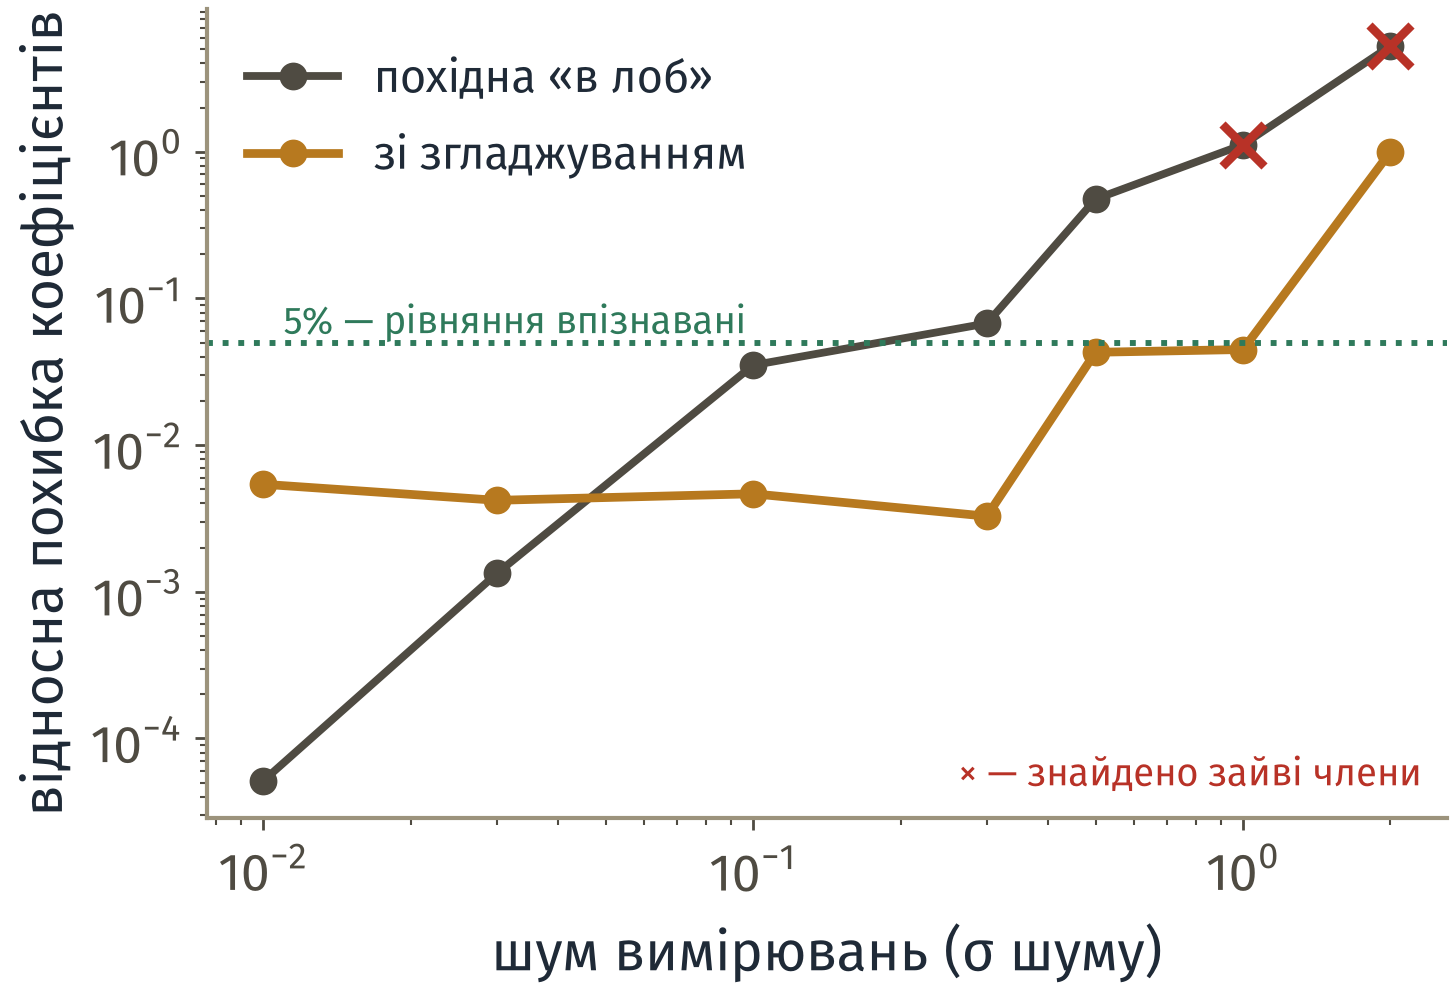
\includegraphics[width=\linewidth]{pop_sindy.png}\\
      \footnotesize\dimtxt{Шум убиває похідні; згладжування рятує до шуму $\sim 1$.}
    \end{column}
  \end{columns}
\end{frame}

\end{document}
